\chapter{Confounding and DAGs}
\section{Confounding}
\subsection{Ignorability and Confounding}
If the ignorability assumption is violated, treatment assignment depends on the potential outcomes. 可以举两个例子.

\begin{ex}
	研究某种药物的治疗效果,$A$表示是否接受治疗,$Y$表示康复人数,$X$表示病情. 病情严重的病人更有可能接受治疗,而病情轻微的病人更可能不采取治疗,因此在treated group,很多都是病情严重的病人,在control group大多数都是病情轻微的病人. 此时治疗的分配并不是随机的,treated group可能因为病情严重没有康复者,control group因为病情轻微可以自愈. 此时的outcome就与治疗的分配有关.
\end{ex}
\begin{ex}
	研究广告投放对未来用户登录量的影响. $A$表示是否被投放广告,$Y$表示未来5日登录人数,$X$表示过去1个月登录次数. 互联网公司更可能会对$X$小的用户投放广告,此时treated group中过去登录次数少的用户占了一大部分,即使对他们投放了广告,他们的$Y$也可能很小. 而control group原本就登录频繁,未来的$Y$也会比较大. 此时的outcome与广告的投放有关.
\end{ex}

从上面的例子我们看到,在treatment assignment与$X$有关时,如果不控制$X$,就违背了ignorability assumption,此时不能识别真实的causal effect.

\subsection{Confounding}
{\color{red} Confounders} are variables that affect both treatment and outcome. 

We note that the effect of $X$ to $Y$ is independent to the treatment. Fig.\ref{cslgph} shows the relationship between confounders, treatment and outcome.

\begin{figure}[htbp]
	\setlength{\abovecaptionskip}{0pt}     %调整图片标题与图距离
	\setlength{\belowcaptionskip}{10pt}
	\vspace{-0cm}  %调整图片与上文的垂直距离
	\setlength{\abovecaptionskip}{-0cm}   %调整图片标题与图距离
	\setlength{\belowcaptionskip}{-0cm}   %调整图片标题与下文距离
	\centering
	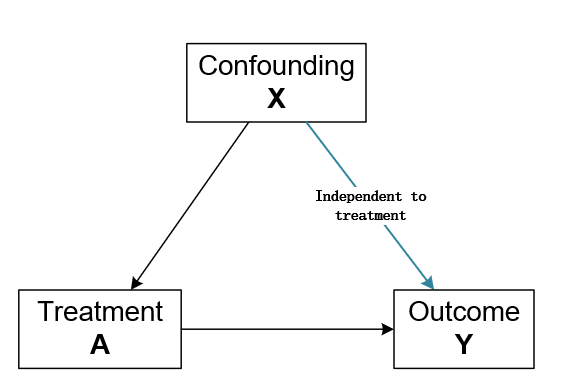
\includegraphics[width=0.4\textwidth]{figure/cslgph.png}
	\caption{Causal graph}
	\label{cslgph}
\end{figure}
	
如果一个变量并不是既影响treatmet又影响outcome,那么这个变量就不是confounder. Fig.\ref{exconfounder}所示.
\begin{figure}[htbp]
	\setlength{\abovecaptionskip}{0pt}     %调整图片标题与图距离
	\setlength{\belowcaptionskip}{10pt}
	\vspace{-0cm}  %调整图片与上文的垂直距离
	\setlength{\abovecaptionskip}{-0cm}   %调整图片标题与图距离
	\setlength{\belowcaptionskip}{-0cm}   %调整图片标题与下文距离
	\centering
	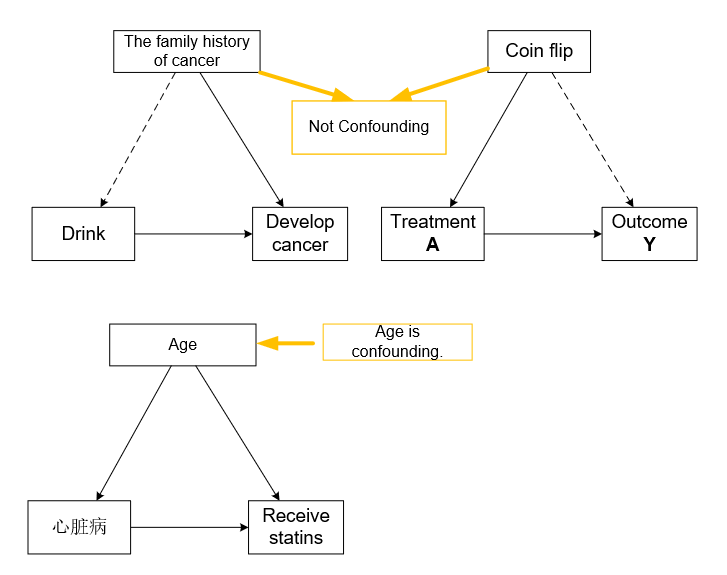
\includegraphics[width=0.8\textwidth]{figure/exconfounder.png}
	\caption{Distinguish confounders}
	\label{exconfounder}
\end{figure}

\subsection{Confounding Control}
\begin{enumerate}[label=(\arabic*)]
	\item {\bfseries 重要性}:Identifying a set of variables $X$, 以保证ignorability assumption成立. {\hl The set of variables is sufficient to control for confounding.}
	\item 用什么方法control this set of variables?
\end{enumerate}

\section{Causal Graph} \label{Causalgraph}
Causal graph: directed acyclic graph.
\subsection{The importance of causal graph}
1. Make assumptions explicit:DAG depicts the assumptions we making on the relationship between variables.

2.Helpful for identifying which variables to control for.

\subsection{Simple graph}
Directed graph $A \longrightarrow Y$: $A$ affects $Y$.

Undirected graph A $\rule[4pt]{0.8cm}{0.05em}$ Y: $A$ is associated with $Y$.\\

\subsection{Graphical models}
\begin{itemize}
	\item 图模型反映了变量之间的independence、dependence、conditional independence的关系. 我们能做的是通过observed data去验证因果图显示的关系是否存在.
	\item 推导非参数的因果效应估计量.(后面会讲到.)
\end{itemize}

\subsection{Terminology}
这一部分讲到了DAG的专业名词:node(vertice), link(edge), path, parent, child, ancestor, descendant.

\paragraph{Path:}与原来认识的path不同. 这里的path并不局限于指向同一方向的路径,指向同一方向的path称为chain,我们后面会讲到另外两种path,称为fork和inverted fork.
\begin{ex}
	在Fig.\ref{expath}中,我们可以找到4条从D到B的path,分别是:\\
	(1) D $\longrightarrow$ A $\longrightarrow$ B; \\
	(2) D $\longrightarrow$ A $\longleftarrow$ G $\longrightarrow$ B;\\
	(3) D $\longrightarrow$ E $\longrightarrow$ G $\longrightarrow$ B;\\
	(4) D $\longrightarrow$ E $\longrightarrow$ G
	$\longrightarrow$ A $\longrightarrow$ B;
\end{ex}
\begin{figure}[htbp]
	\setlength{\abovecaptionskip}{0pt}     %调整图片标题与图距离
	\setlength{\belowcaptionskip}{10pt}
	\vspace{-0cm}  %调整图片与上文的垂直距离
	\setlength{\abovecaptionskip}{-0cm}   %调整图片标题与图距离
	\setlength{\belowcaptionskip}{-0cm}   %调整图片标题与下文距离
	\centering
	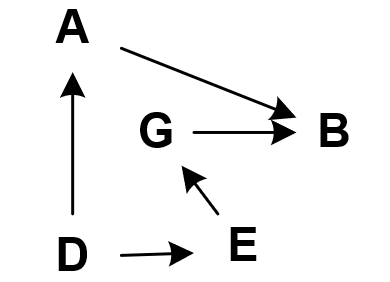
\includegraphics[width=0.2\textwidth]{figure/expath.png}
	\caption{Example of paths}
	\label{expath}
\end{figure}

\paragraph{Parents and ancestors} we look at a chain in Fig.\ref{expath}: 
\begin{equation}
D \longrightarrow E \longrightarrow G.
\end{equation}
	
	In this chain, E is the child of D, and D is the parent of E. D and E are the ancestors of G, and E and G are the descendants of D.


\subsection{DAGs}
DAGs的条件:
\begin{itemize}
	\item 不存在undirected edge.
	\item No circle.
\end{itemize}

\subsection{conclusion}
最后总结一下这一课的重点:
\begin{figure}[htbp]
	\setlength{\abovecaptionskip}{0pt}     %调整图片标题与图距离
	\setlength{\belowcaptionskip}{10pt}
	\vspace{-0cm}  %调整图片与上文的垂直距离
	\setlength{\abovecaptionskip}{-0cm}   %调整图片标题与图距离
	\setlength{\belowcaptionskip}{-0cm}   %调整图片标题与下文距离
	\centering
	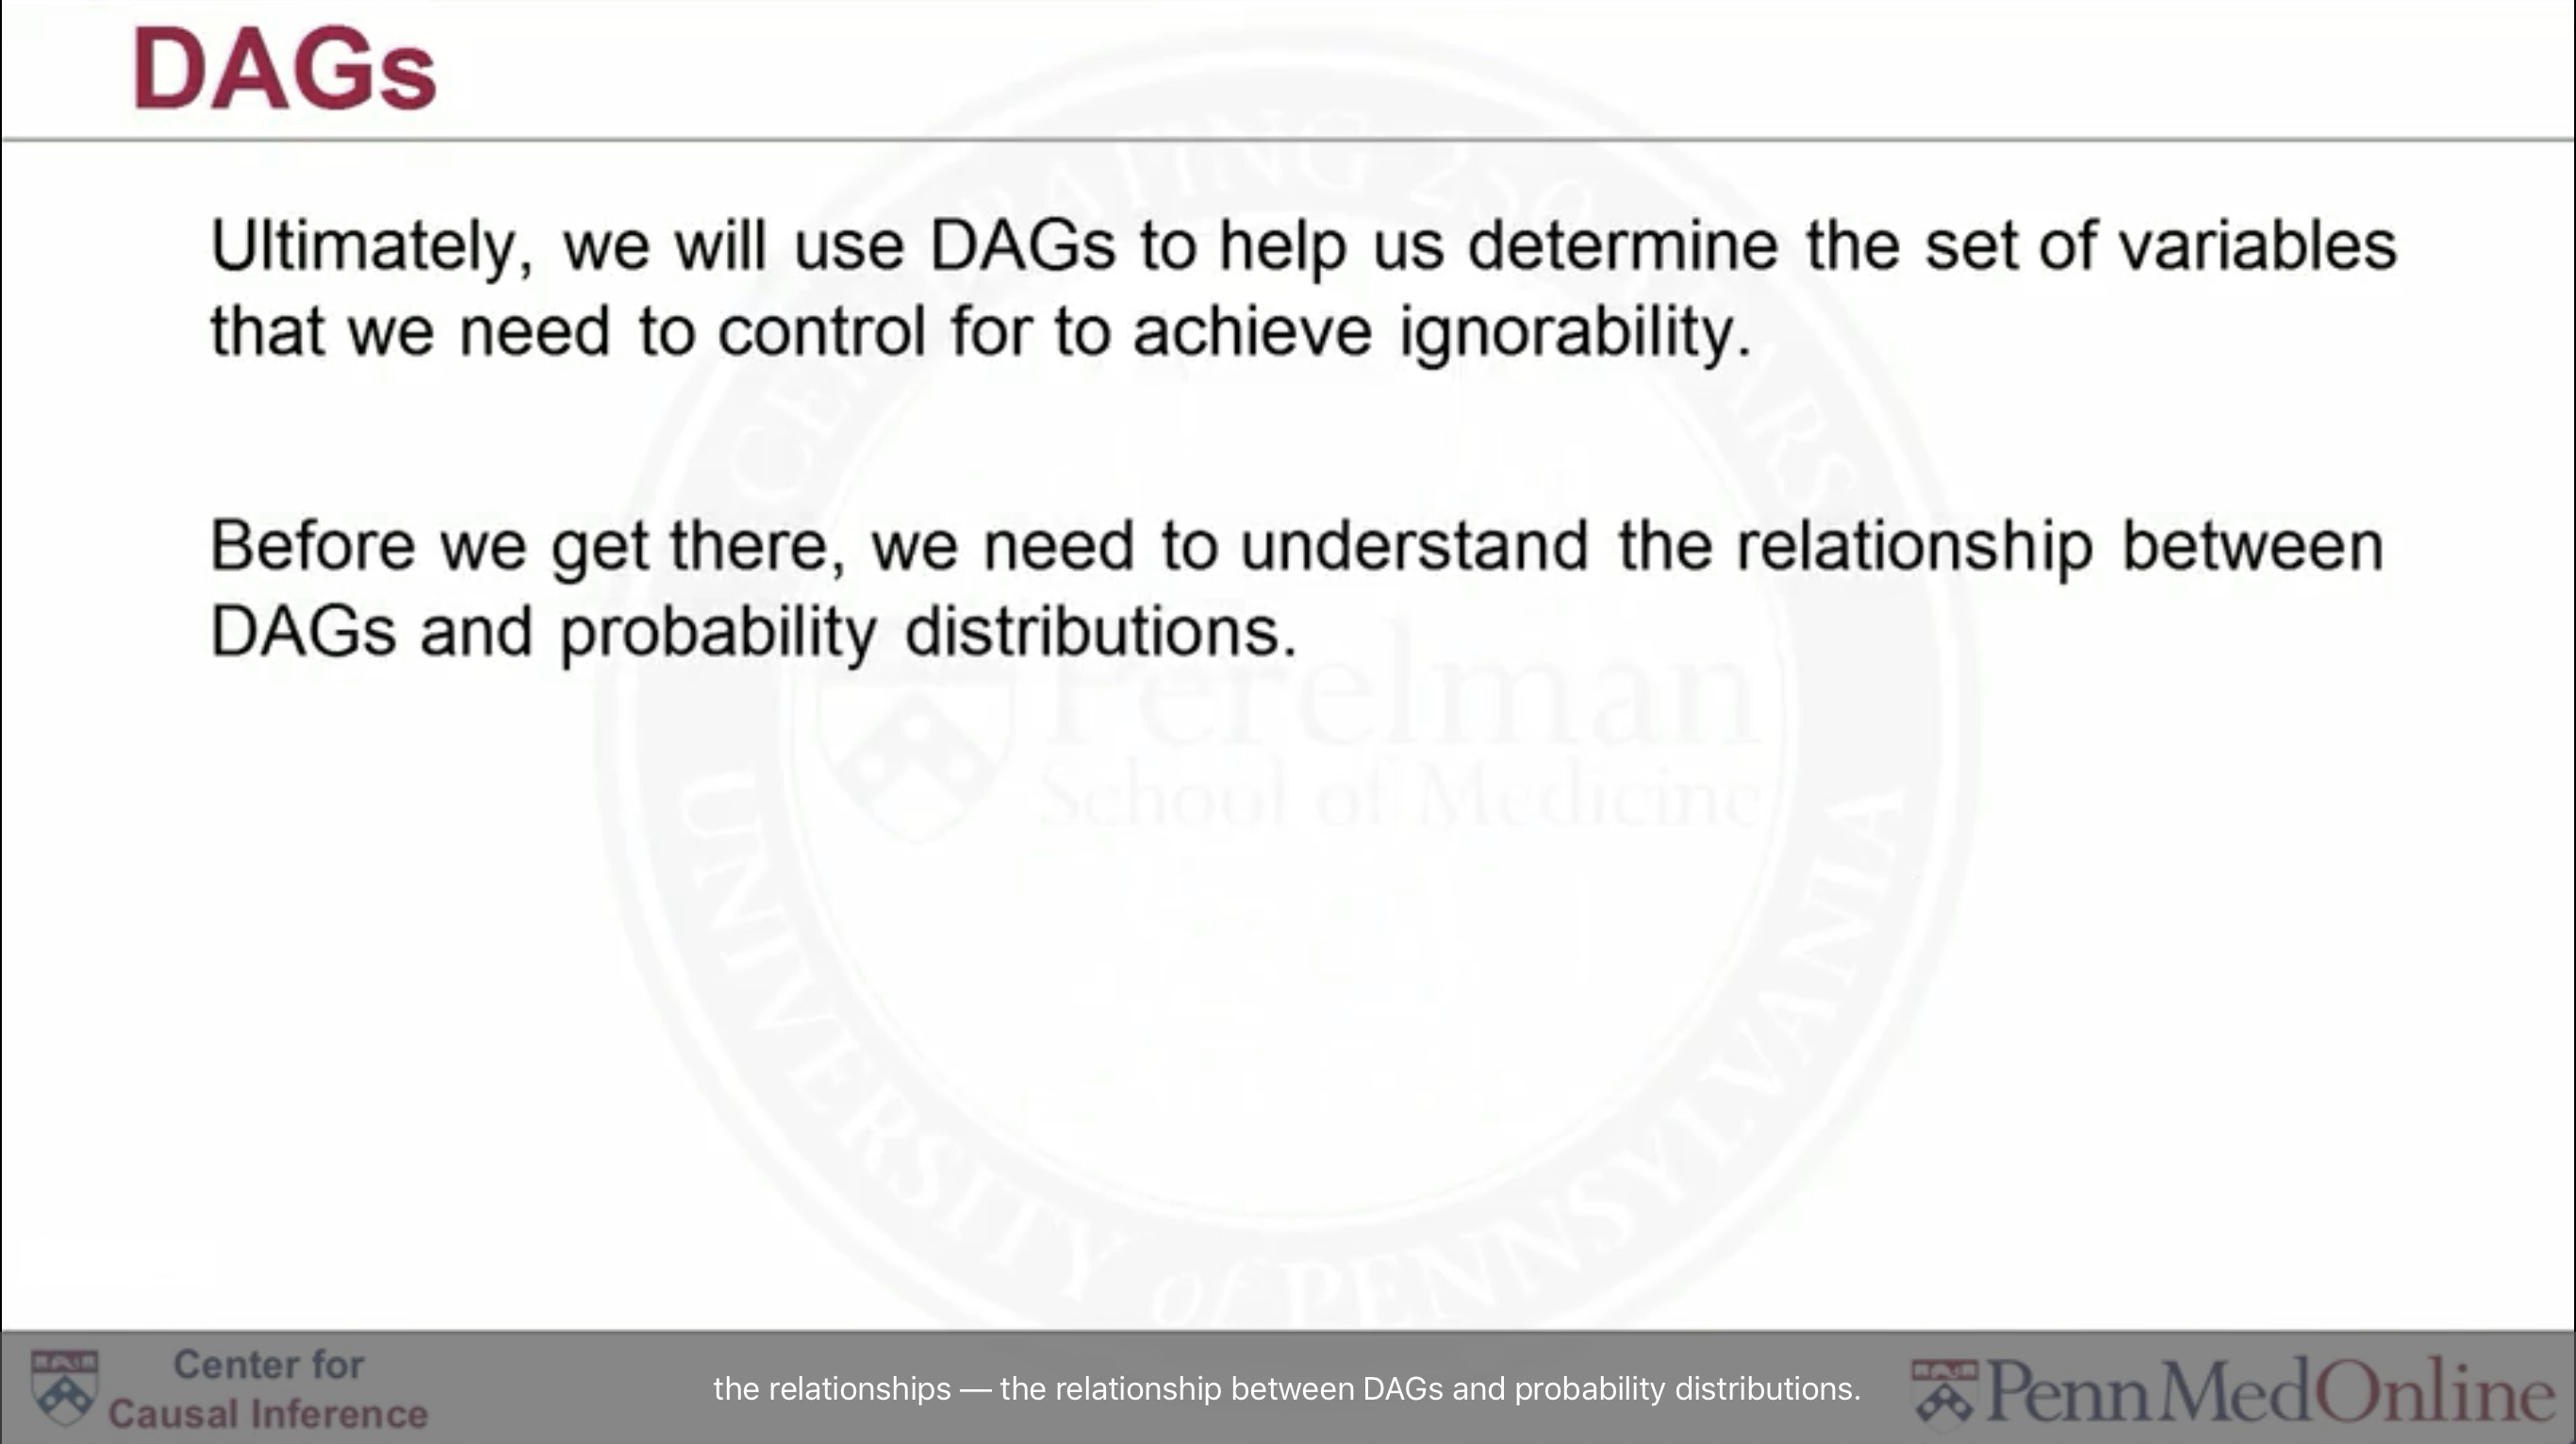
\includegraphics[width=0.8\textwidth]{figure/dagconclusion.jpg}
	\caption{Conclusion of DAGs}
	\label{dagconclusion}
\end{figure}


\newpage \section{Relationship between DAGs and probability distributions}
\noindent {\bfseries Outline:}\\
1. The relationship between DAGs and probability distributions.\\
2. Decomposition of joint distribution.\\
3. Compatibility of DAGs and probability.
\subsection{The relationship between DAGs and probability distributions} 
在\ref{Causalgraph}中,我们说到DAG可以反映出variables之间的independence, dependence, conditional independence关系. 对于DAG中的所有nodes,DAG编码了它们之间joint distribution的假设. 下面举例说明DAG能向我们传达什么信息.
\begin{ex}
	从Fig.\ref{DAGex1}的因果图中,我们可以解码出4个节点的联合分布信息:
    \begin{itemize}
    	\item P(C$|$A,B,D) = P(C), i.e., C与A,B,D独立. Conditional on A,B,D, does not tell any information about the probability of C.
        {\b \item P(A$|$B,C,D) = P(A$|$B,D) }
    	\item P(B$|$A,C,D) = P(B$|$A,D)=p(B$|$A), i.e., B$\perp$D$|$A. D对B的影响都是通过A作用的,当给定A时,D对A的作用也包含在A里面了,此时D不再给B的分布提供额外的信息.
    	\item P(B$|$D) $\neq$ P(B), B and D are (marginally) dependent. 在上一则item中我们知道给定A时,B和D是条件独立的. 然而尽管D对B的作用不是直接的,但是D与B却是边缘相关的. {\color{orange} 可以这样理解:把D的作用从B中控制住,剩余部分的分布很明显不能等于原始B的分布.}	
    	\item P(D$|$A,B,C) = P(D$|$A,B) = P(D$|$A), B与D的相关是通过A的,给定A之后,B就不能对D的分布提供额外信息了.
    \end{itemize}
\end{ex}
	\begin{figure}[htbp]
	\setlength{\abovecaptionskip}{0pt}     %调整图片标题与图距离
	\setlength{\belowcaptionskip}{10pt}
	\vspace{-0cm}  %调整图片与上文的垂直距离
	\setlength{\abovecaptionskip}{-0cm}   %调整图片标题与图距离
	\setlength{\belowcaptionskip}{-0cm}   %调整图片标题与下文距离
	\centering
	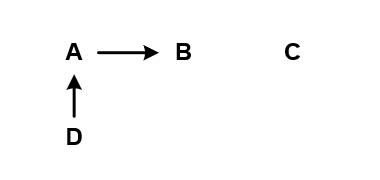
\includegraphics[width=0.4\textwidth]{figure/DAGex1.png}
	\caption{Example 1}
	\label{DAGex1}
    \end{figure}

\begin{ex}
	从Fig.\ref{DAGex2}的因果图中,我们可以解码出4个节点的联合分布信息:
	\begin{itemize}
		\item P(A$|$B,C,D) = P(A$|$D), 对A产生影响的只有D,给定D,我们就知道了关于A的所有.
		\item P(D$|$A,B,C) = P(D$|$A,B), {\color{red} D对A,B分别有独立的影响,所以A,B之中独立地蕴含了与D有关的信息.} {\color{orange} 虽然C与D也有关系,但是是通过B作用的,给定B之后,C中就不包含对D有用的信息了.}
	\end{itemize}
\end{ex}

	
	\begin{figure}[htbp]
	\setlength{\abovecaptionskip}{0pt}     %调整图片标题与图距离
	\setlength{\belowcaptionskip}{10pt}
	\vspace{-0cm}  %调整图片与上文的垂直距离
	\setlength{\abovecaptionskip}{-0cm}   %调整图片标题与图距离
	\setlength{\belowcaptionskip}{-0cm}   %调整图片标题与下文距离
	\centering
	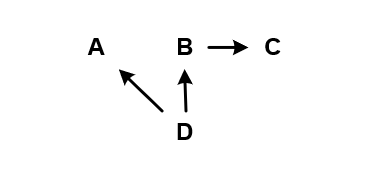
\includegraphics[width=0.4\textwidth]{figure/DAGex2.png}
	\caption{Example 2}
	\label{DAGex2}
    \end{figure}


\begin{ex}
	从Fig.\ref{DAGex3}的因果图中,我们可以解码出4个节点的联合分布信息:
    \begin{itemize}
    	\item P(A$|$B,C,D) = P(A$|$C,D),从path的角度来讲, B到A没有path, 可以直接把B去掉.
    	\item P(D$|$A,B,C) = P(D$|$A,B), 从path的角度来讲,C对D的影响都是通过A和B的,给了A和B之后,C中就不包含对D的分布有用的信息了.
    \end{itemize}
\end{ex}

	\begin{figure}[htbp]
	\setlength{\abovecaptionskip}{0pt}     %调整图片标题与图距离
	\setlength{\belowcaptionskip}{10pt}
	\vspace{-0cm}  %调整图片与上文的垂直距离
	\setlength{\abovecaptionskip}{-0cm}   %调整图片标题与图距离
	\setlength{\belowcaptionskip}{-0cm}   %调整图片标题与下文距离
	\centering
	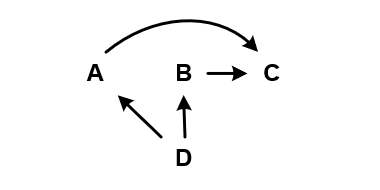
\includegraphics[width=0.4\textwidth]{figure/DAGex3.png}
	\caption{Example 3}
	\label{DAGex3}
\end{figure}

\subsection{Decomposition fo Joint Distribution}
在上面的3个例子,将节点的联合分布分解: 
\begin{enumerate}[label=(\arabic*)]
	\item P(A,B,C,D) = P(B$|$A)P(A$|$D)P(D)P(C)
	\item P(A,B,C,D) = P(C$|$B)P(B$|$D)P(A$|$D)P(D)
    \item P(A,B,C,D) = P(C$|$A,B)P(A$|$D)P(B$|$D)P(D)
\end{enumerate}

\subsection{Compatibility}
这一部分探讨的是DAG与Probability function能不能{\bfseries 互推}. 举个例子.
\begin{ex}
Probability distribution: P(A,B) $ \neq$ P(A)P(B). There are 2 DAGs compatible with this probability:
A $\longrightarrow$ B, and A $\longleftarrow $B.
\end{ex}

说明{\color{red}一个probability function对应的DAG并不是唯一的}.
因此我们使用DAG来表示变量关系,而不是probability function.


\newpage\section{Paths and associations}
\subsection{Types of Paths}
(1) Fork: information flows from one node to different nodes. Fig.\ref{fork} shows the basic structure of fork.
	\begin{figure}[htbp]
	\setlength{\abovecaptionskip}{0pt}     %调整图片标题与图距离
	\setlength{\belowcaptionskip}{10pt}
	\vspace{-0cm}  %调整图片与上文的垂直距离
	\setlength{\abovecaptionskip}{-0cm}   %调整图片标题与图距离
	\setlength{\belowcaptionskip}{-0cm}   %调整图片标题与下文距离
	\centering
	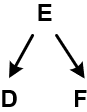
\includegraphics[width=0.1\textwidth]{figure/fork.png}
	\caption{Fork}
	\label{fork}
    \end{figure}

(2) Chain: information flows in one direction. Fig.\ref{chain} shows the basic structure of chain.
	\begin{figure}[htbp]
	\setlength{\abovecaptionskip}{0pt}     %调整图片标题与图距离
	\setlength{\belowcaptionskip}{10pt}
	\vspace{-0cm}  %调整图片与上文的垂直距离
	\setlength{\abovecaptionskip}{-0cm}   %调整图片标题与图距离
	\setlength{\belowcaptionskip}{-0cm}   %调整图片标题与下文距离
	\centering
	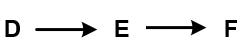
\includegraphics[width=0.2\textwidth]{figure/chain.png}
	\caption{Chain}
	\label{chain}
    \end{figure}

(3)Inverted forks: Information flows from different nodes to one node. 
	\begin{figure}[htbp]
	\setlength{\abovecaptionskip}{0pt}     %调整图片标题与图距离
	\setlength{\belowcaptionskip}{10pt}
	\vspace{-0cm}  %调整图片与上文的垂直距离
	\setlength{\abovecaptionskip}{-0cm}   %调整图片标题与图距离
	\setlength{\belowcaptionskip}{-0cm}   %调整图片标题与下文距离
	\centering
	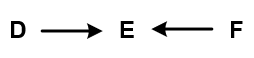
\includegraphics[width=0.2\textwidth]{figure/invfork.png}
	\caption{Inverted fork}
	\label{invfork}
    \end{figure}
In Fig.\ref{invfork}, "E" is called as "Collider". It's the junction of information.

\subsection{Relationship between varaibles in 3 types of paths}
(1) {\bfseries Induce dependence of E and F:} Fork and chain. 
\begin{itemize}
	\item In fork path, the information in E flows to both D and F, so D and F are dependent.  
	\item In chain path, the information in D flows to E and then flows to F. Or we can say that D affects E and then E affects F. So E and F are obviously dependent. {\g  {Most importantly, it is E that really causing this association between D and F.}}
\end{itemize}

(2) {\bfseries Induce independece of E and F:} Inverted fork. 
\begin{itemize}
	\item There is no information flows to E from F, and there is also no information flows to F from E. So E and F are independent.
\end{itemize}

\section{Conditional independence(d-separation)}
\subsection{Blocking}
Path can be blocked by conditioning on nodes in the path.

\subsection{Blocking on chain}
Consider the path: $A \longrightarrow G\longrightarrow B$. 

A and B are dependent, but they are dependent through G, A affects G and then G affects B. So it is G that really causing this association between A and B. 

If we condition on the node in the middle of the chain, i.e.,G, we block the path from A to B. {\r {Then A is independent with B.} }

\begin{ex}
Suppose in the given chain path above,  A is temperature. G is whether sidewalk icy or not. B is whether someone falls or not. 

Temperature affects whether the sidewalk is icy or not. And the sidewalk is icy or not affects if someone falls. So temperature is associated with whether someone falls.

Now if we condition on G, say, the sidewalk is icy, then whether someone falling down is not associated with temperature. 
\end{ex}
这告诉我们,控制一条chain path中间的nodes,可以阻断两端nodes的相关性(association).

\subsection{Blocking on fork}
Consider in the fork: $A \longleftarrow G \longrightarrow B$.
We condition on G, making G the same for everyone. Then there is no relationship between A, G and B, i.e., G is no longer affecting A and B because we're holding it fixed.

If we condition on G, the association between A and B is blocked. 

\subsection{Blocking on inverted fork}
{\color{red} The opposite situation occurs if a collider is conditioned on.}
Consider the inverted fork path: $A \longrightarrow G \longleftarrow B$.

A and B are independent in the path, but conditioning on G induces an association between A and B.

\begin{ex}
	Here we give an example as shown in Fig.\ref{blockcollider1} and Fig.\ref{blockcollider2}. 
		\begin{figure}[htbp]
		\setlength{\abovecaptionskip}{0pt}     %调整图片标题与图距离
		\setlength{\belowcaptionskip}{10pt}
		\vspace{-0cm}  %调整图片与上文的垂直距离
		\setlength{\abovecaptionskip}{-0cm}   %调整图片标题与图距离
		\setlength{\belowcaptionskip}{-0cm}   %调整图片标题与下文距离
		\centering
		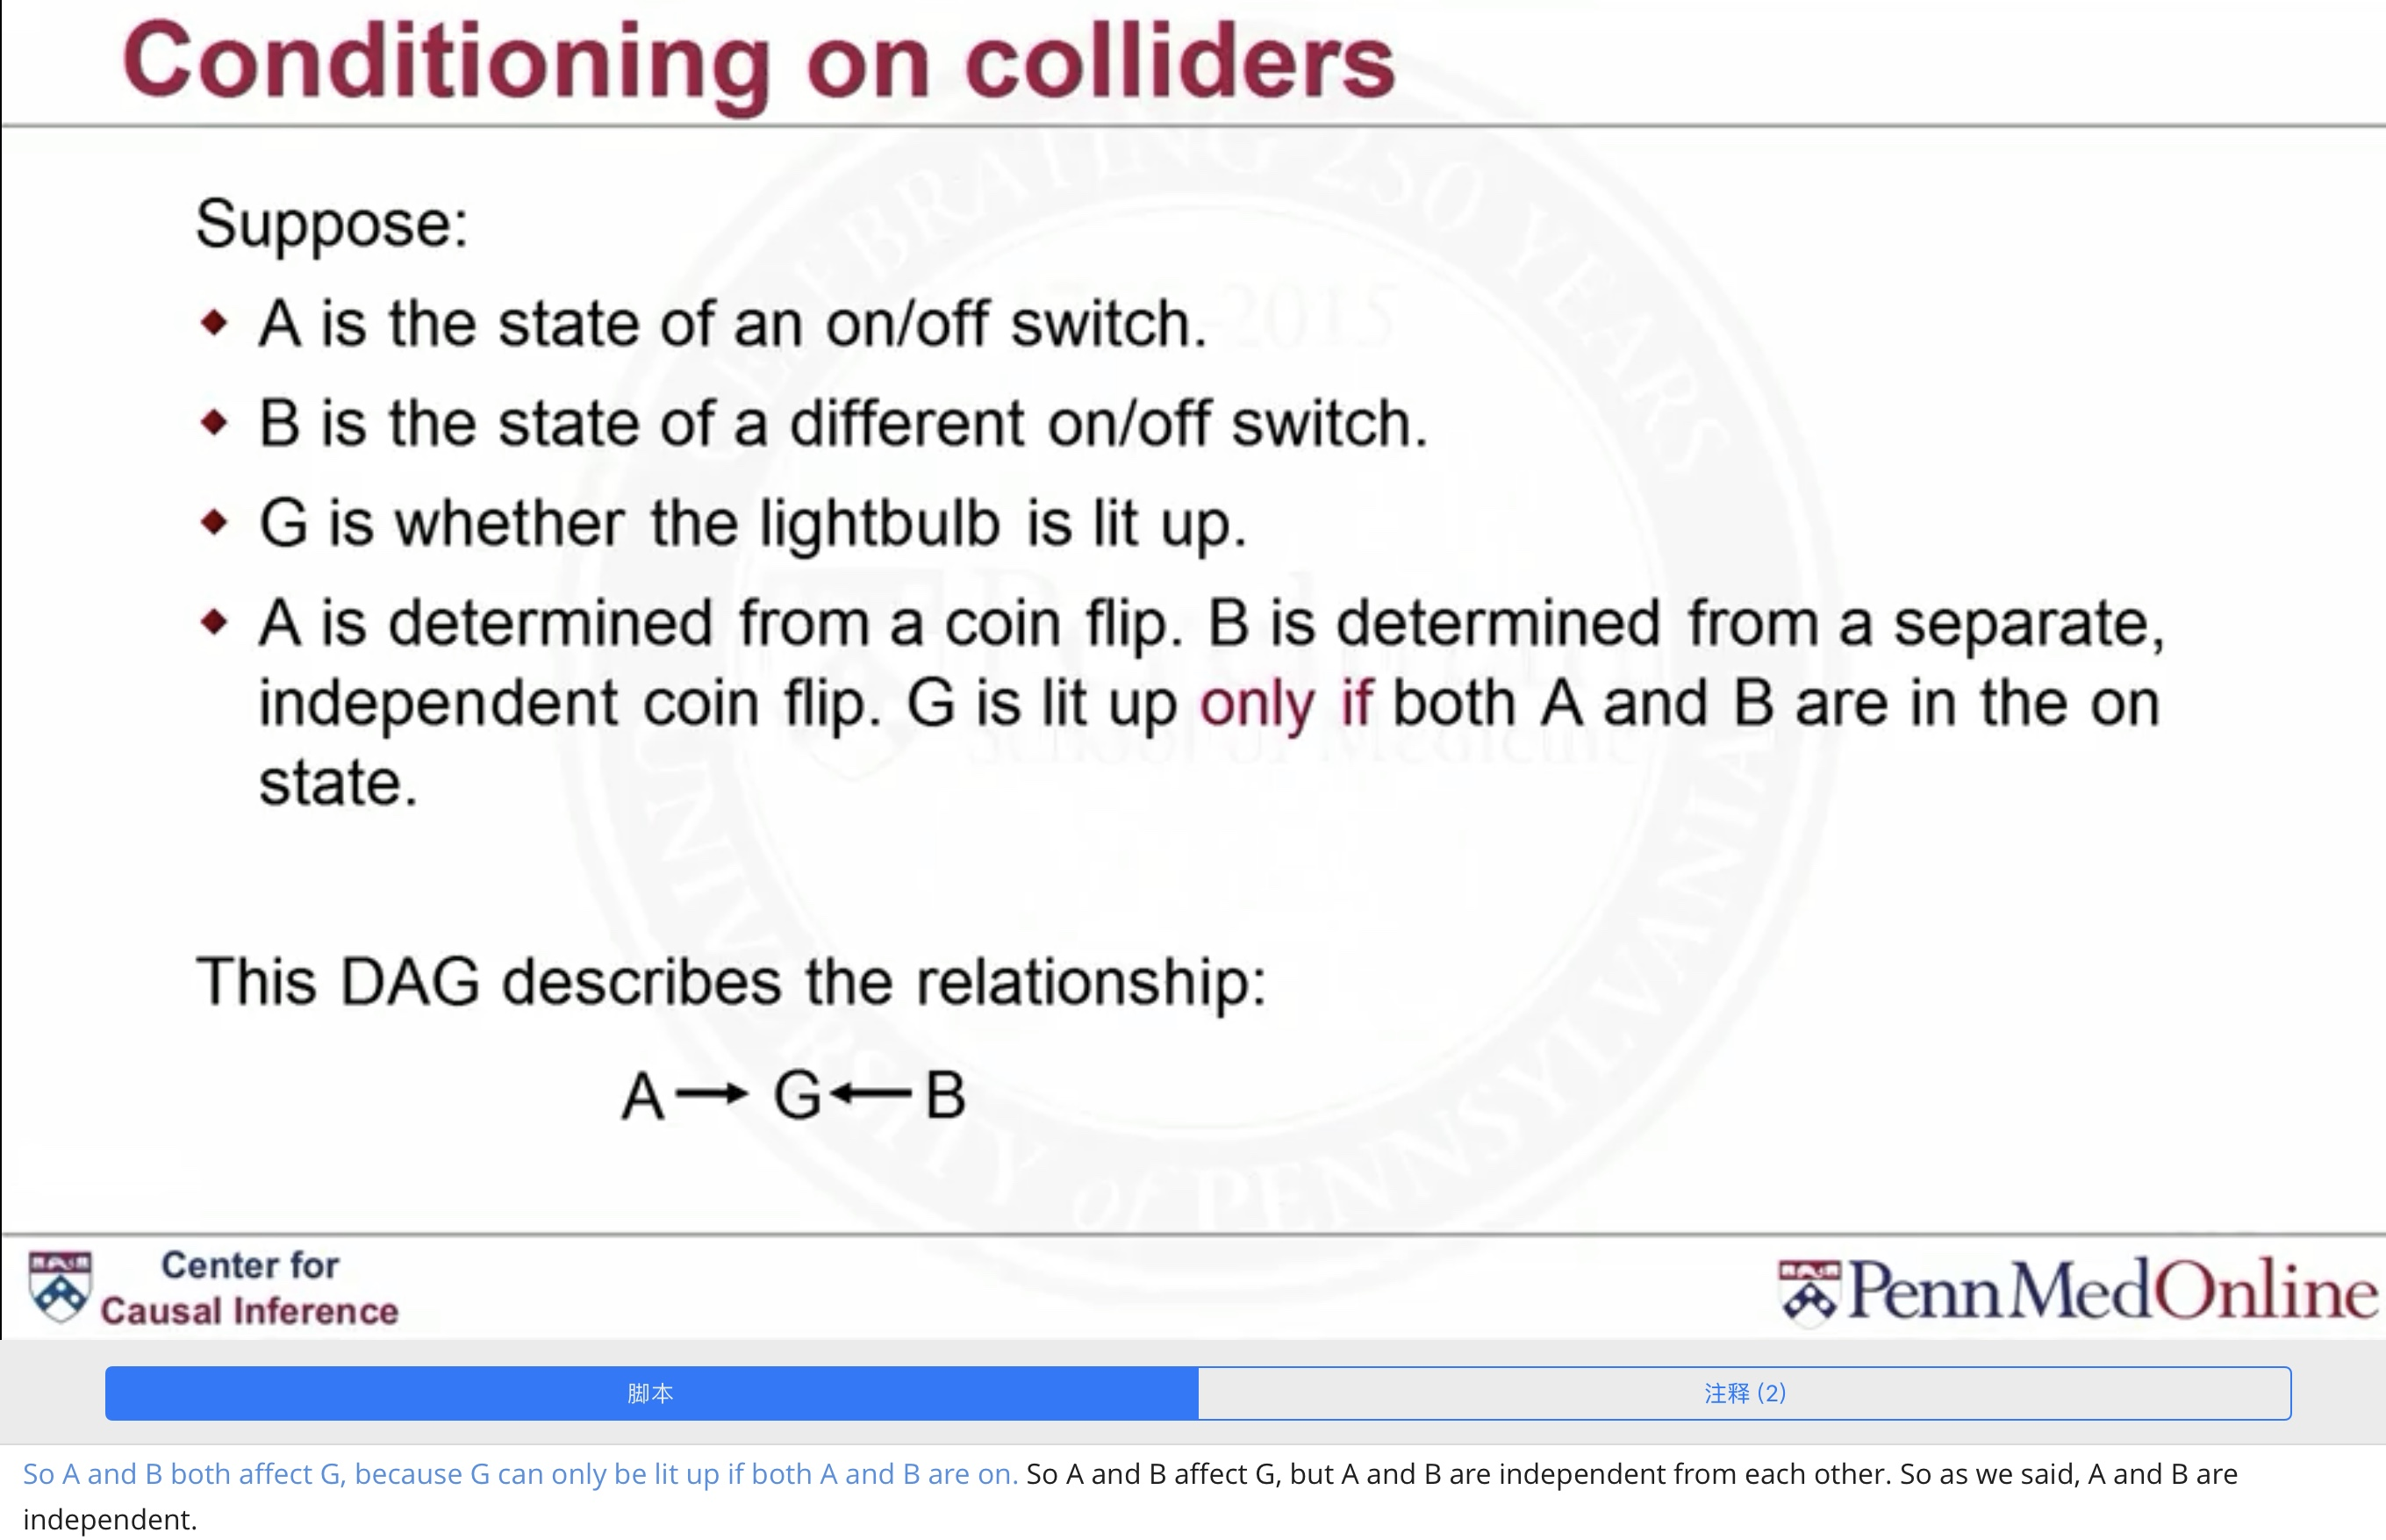
\includegraphics[width=0.8\textwidth]{figure/blockcollider1.jpg}
		\caption{Conditioning on collider(1)}
		\label{blockcollider1}
	\end{figure}

	\begin{figure}[htbp]
	\setlength{\abovecaptionskip}{0pt}     %调整图片标题与图距离
	\setlength{\belowcaptionskip}{10pt}
	\vspace{-0cm}  %调整图片与上文的垂直距离
	\setlength{\abovecaptionskip}{-0cm}   %调整图片标题与图距离
	\setlength{\belowcaptionskip}{-0cm}   %调整图片标题与下文距离
	\centering
	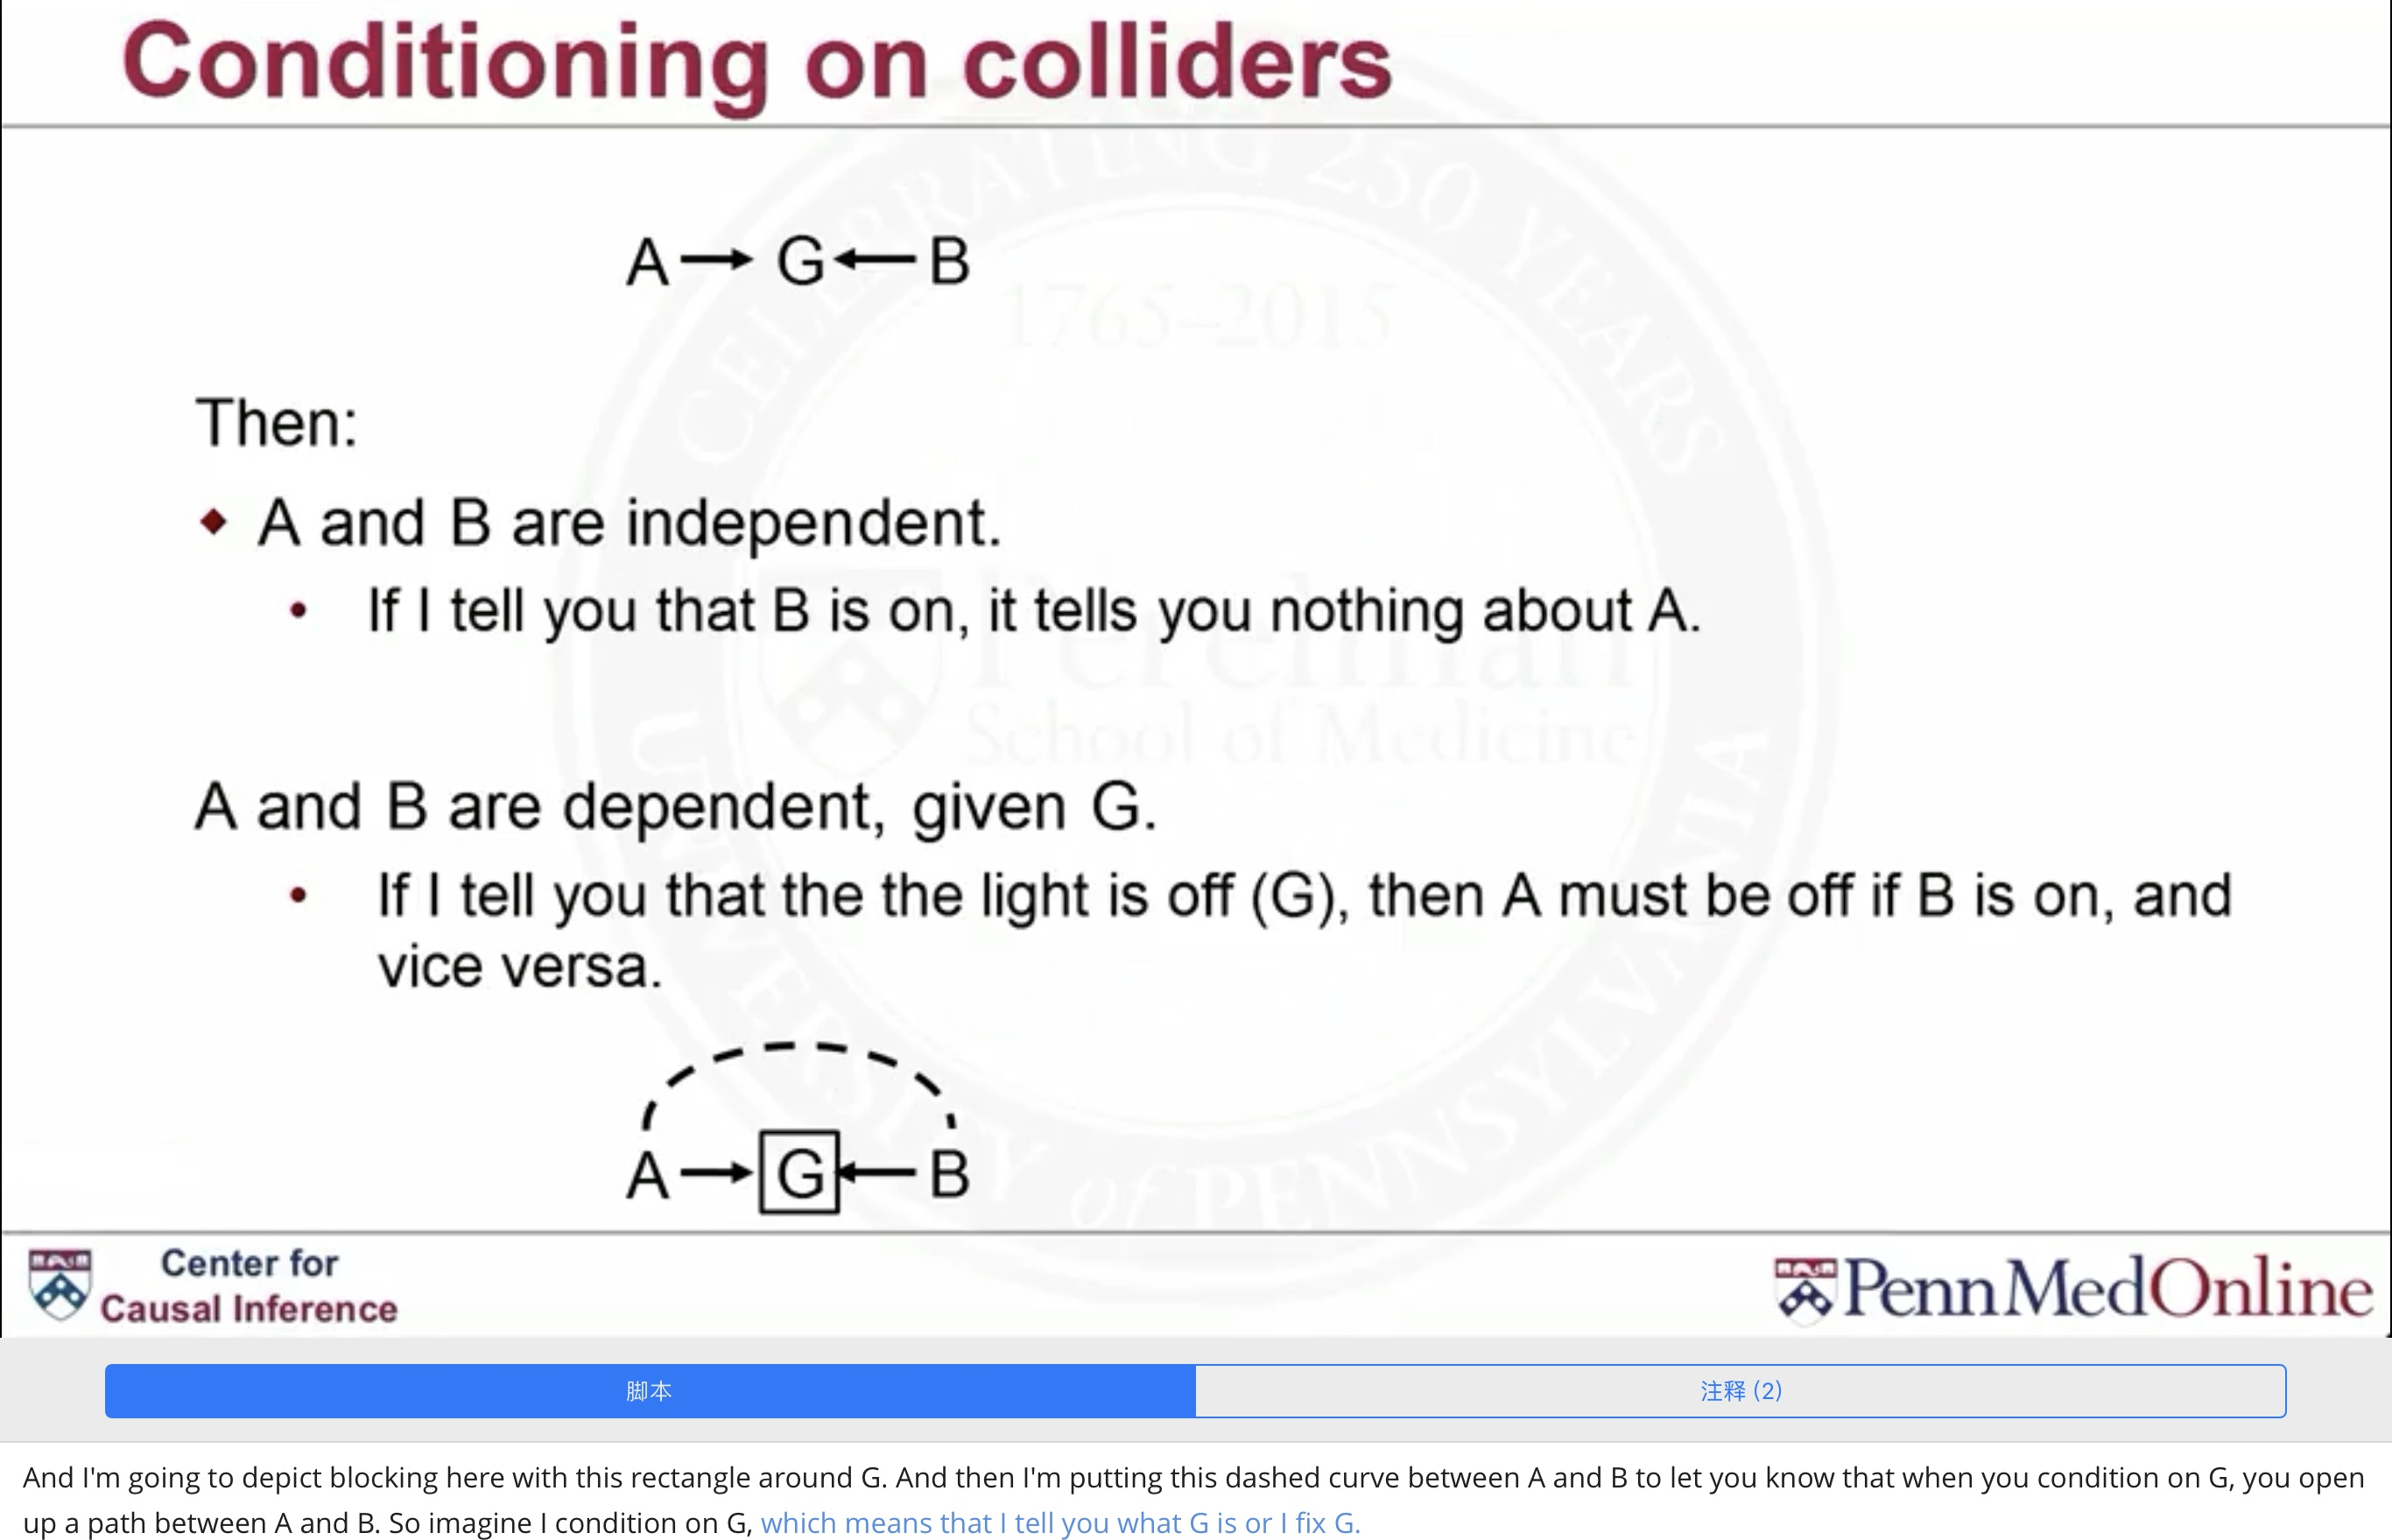
\includegraphics[width=0.8\textwidth]{figure/blockcollider2.jpg}
	\caption{Conditioning on collider(2)}
	\label{blockcollider2}
\end{figure}
	
\end{ex}

\subsection{Conclusion}
\begin{itemize}
	\item Controlling middle part of {\r {fork and chain}} will remove dependence. 
	\item Controlling collider of {\r {inverted fork}} will induce dependence. 
\end{itemize}



\section{Confounding revisited}
\noindent {\bfseries Outline:} \\
1. Frontdoor paths. \\
2. Backdoor paths. Why backdoor path needs to be blocked?

\subsection{Frontdoor path}
{\bfseries Frontdoor path is path that from treatment A to outcome Y. }There may be several nodes in the middle of the path from A to Y. A $\longrightarrow$ Z $\longrightarrow$ Y. As shown in Fig.\ref{frontdoor}.
	\begin{figure}[htbp]
	\setlength{\abovecaptionskip}{0pt}     %调整图片标题与图距离
	\setlength{\belowcaptionskip}{10pt}
	\vspace{-0cm}  %调整图片与上文的垂直距离
	\setlength{\abovecaptionskip}{-0cm}   %调整图片标题与图距离
	\setlength{\belowcaptionskip}{-0cm}   %调整图片标题与下文距离
	\centering
	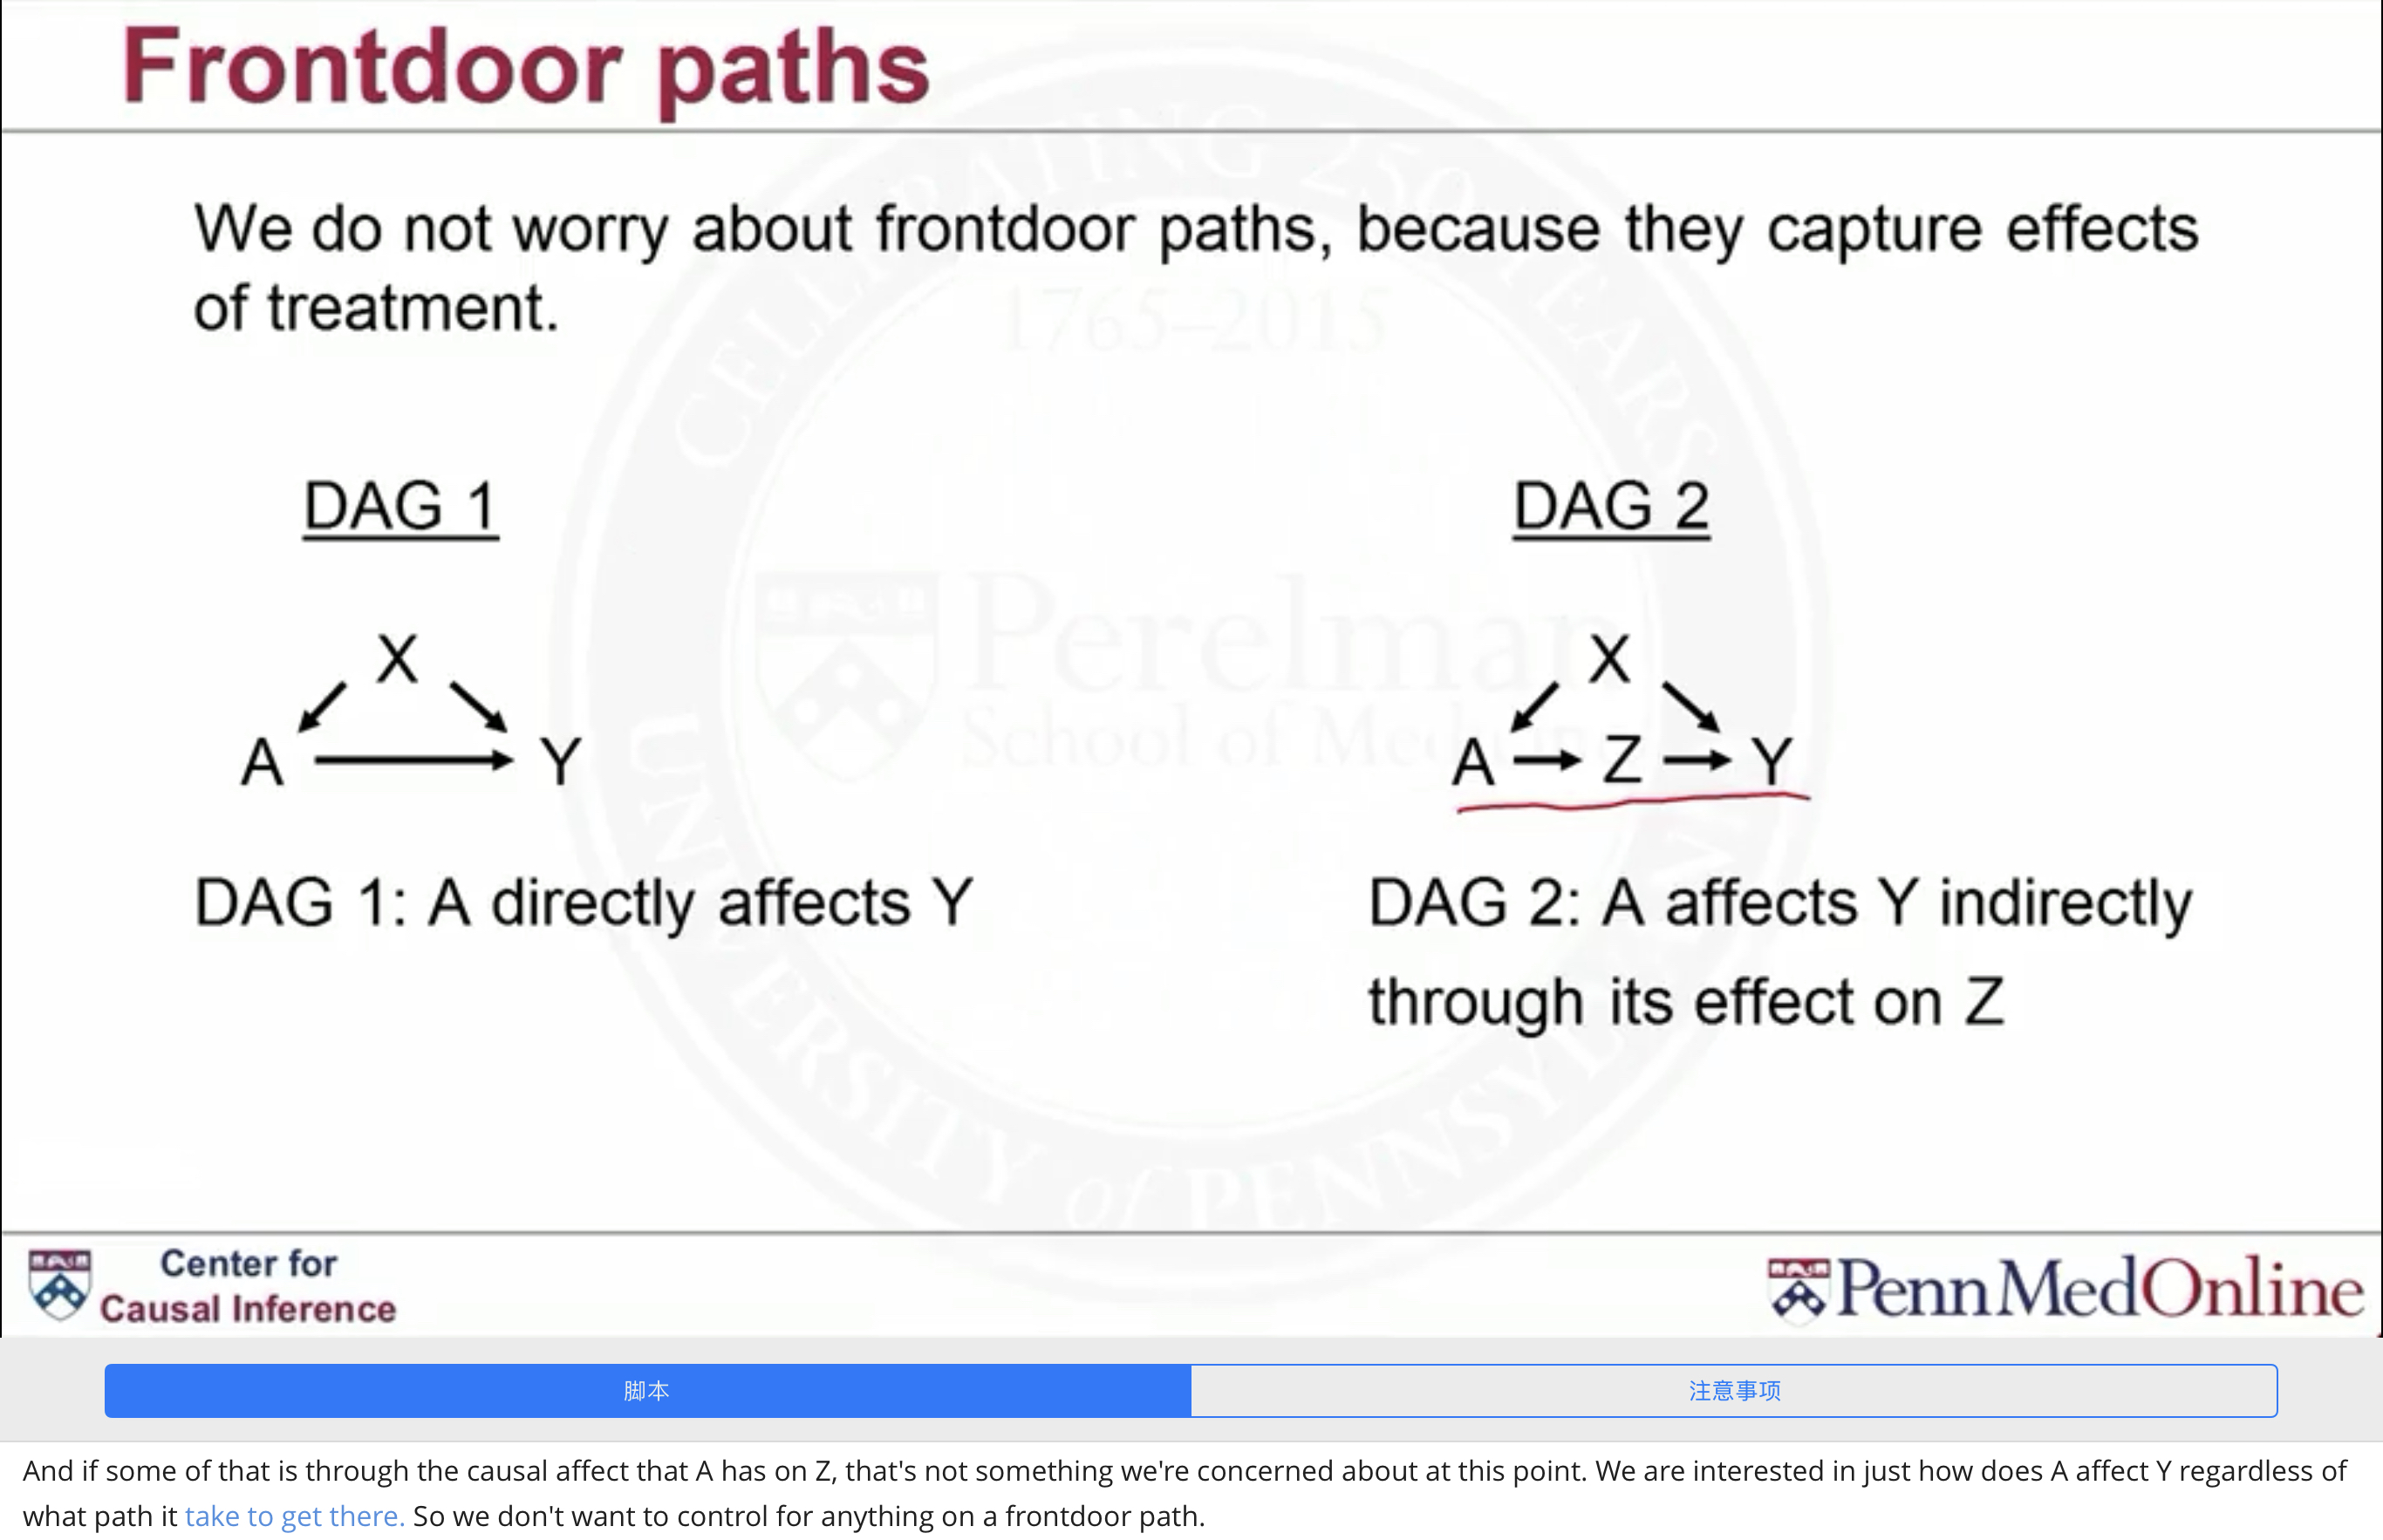
\includegraphics[width=0.8\textwidth]{figure/frontdoor.jpg}
	\caption{Frontdoor path}
	\label{frontdoor}
    \end{figure}
我们感兴趣的是A对Y的causal effect,而不在意A是通过什么作用到Y的. {\bfseries 就算A对Y的causal effect中有一部分是通过A对Z的causal effect实现的,也没有关系. } 我们并不关注这一部分,也就是说 {\color{red} 我们并不需要Control在frontdoor path上出现的variables.}

\subsection{Backdoor path}
{\bfseries Backdoor path is path that from treatment A to Y that travel through arrows {\color{orange}going into} A.}  As shown in Fig.\ref{backdoor}.
	\begin{figure}[htbp]
	\setlength{\abovecaptionskip}{0pt}     %调整图片标题与图距离
	\setlength{\belowcaptionskip}{10pt}
	\vspace{-0cm}  %调整图片与上文的垂直距离
	\setlength{\abovecaptionskip}{-0cm}   %调整图片标题与图距离
	\setlength{\belowcaptionskip}{-0cm}   %调整图片标题与下文距离
	\centering
	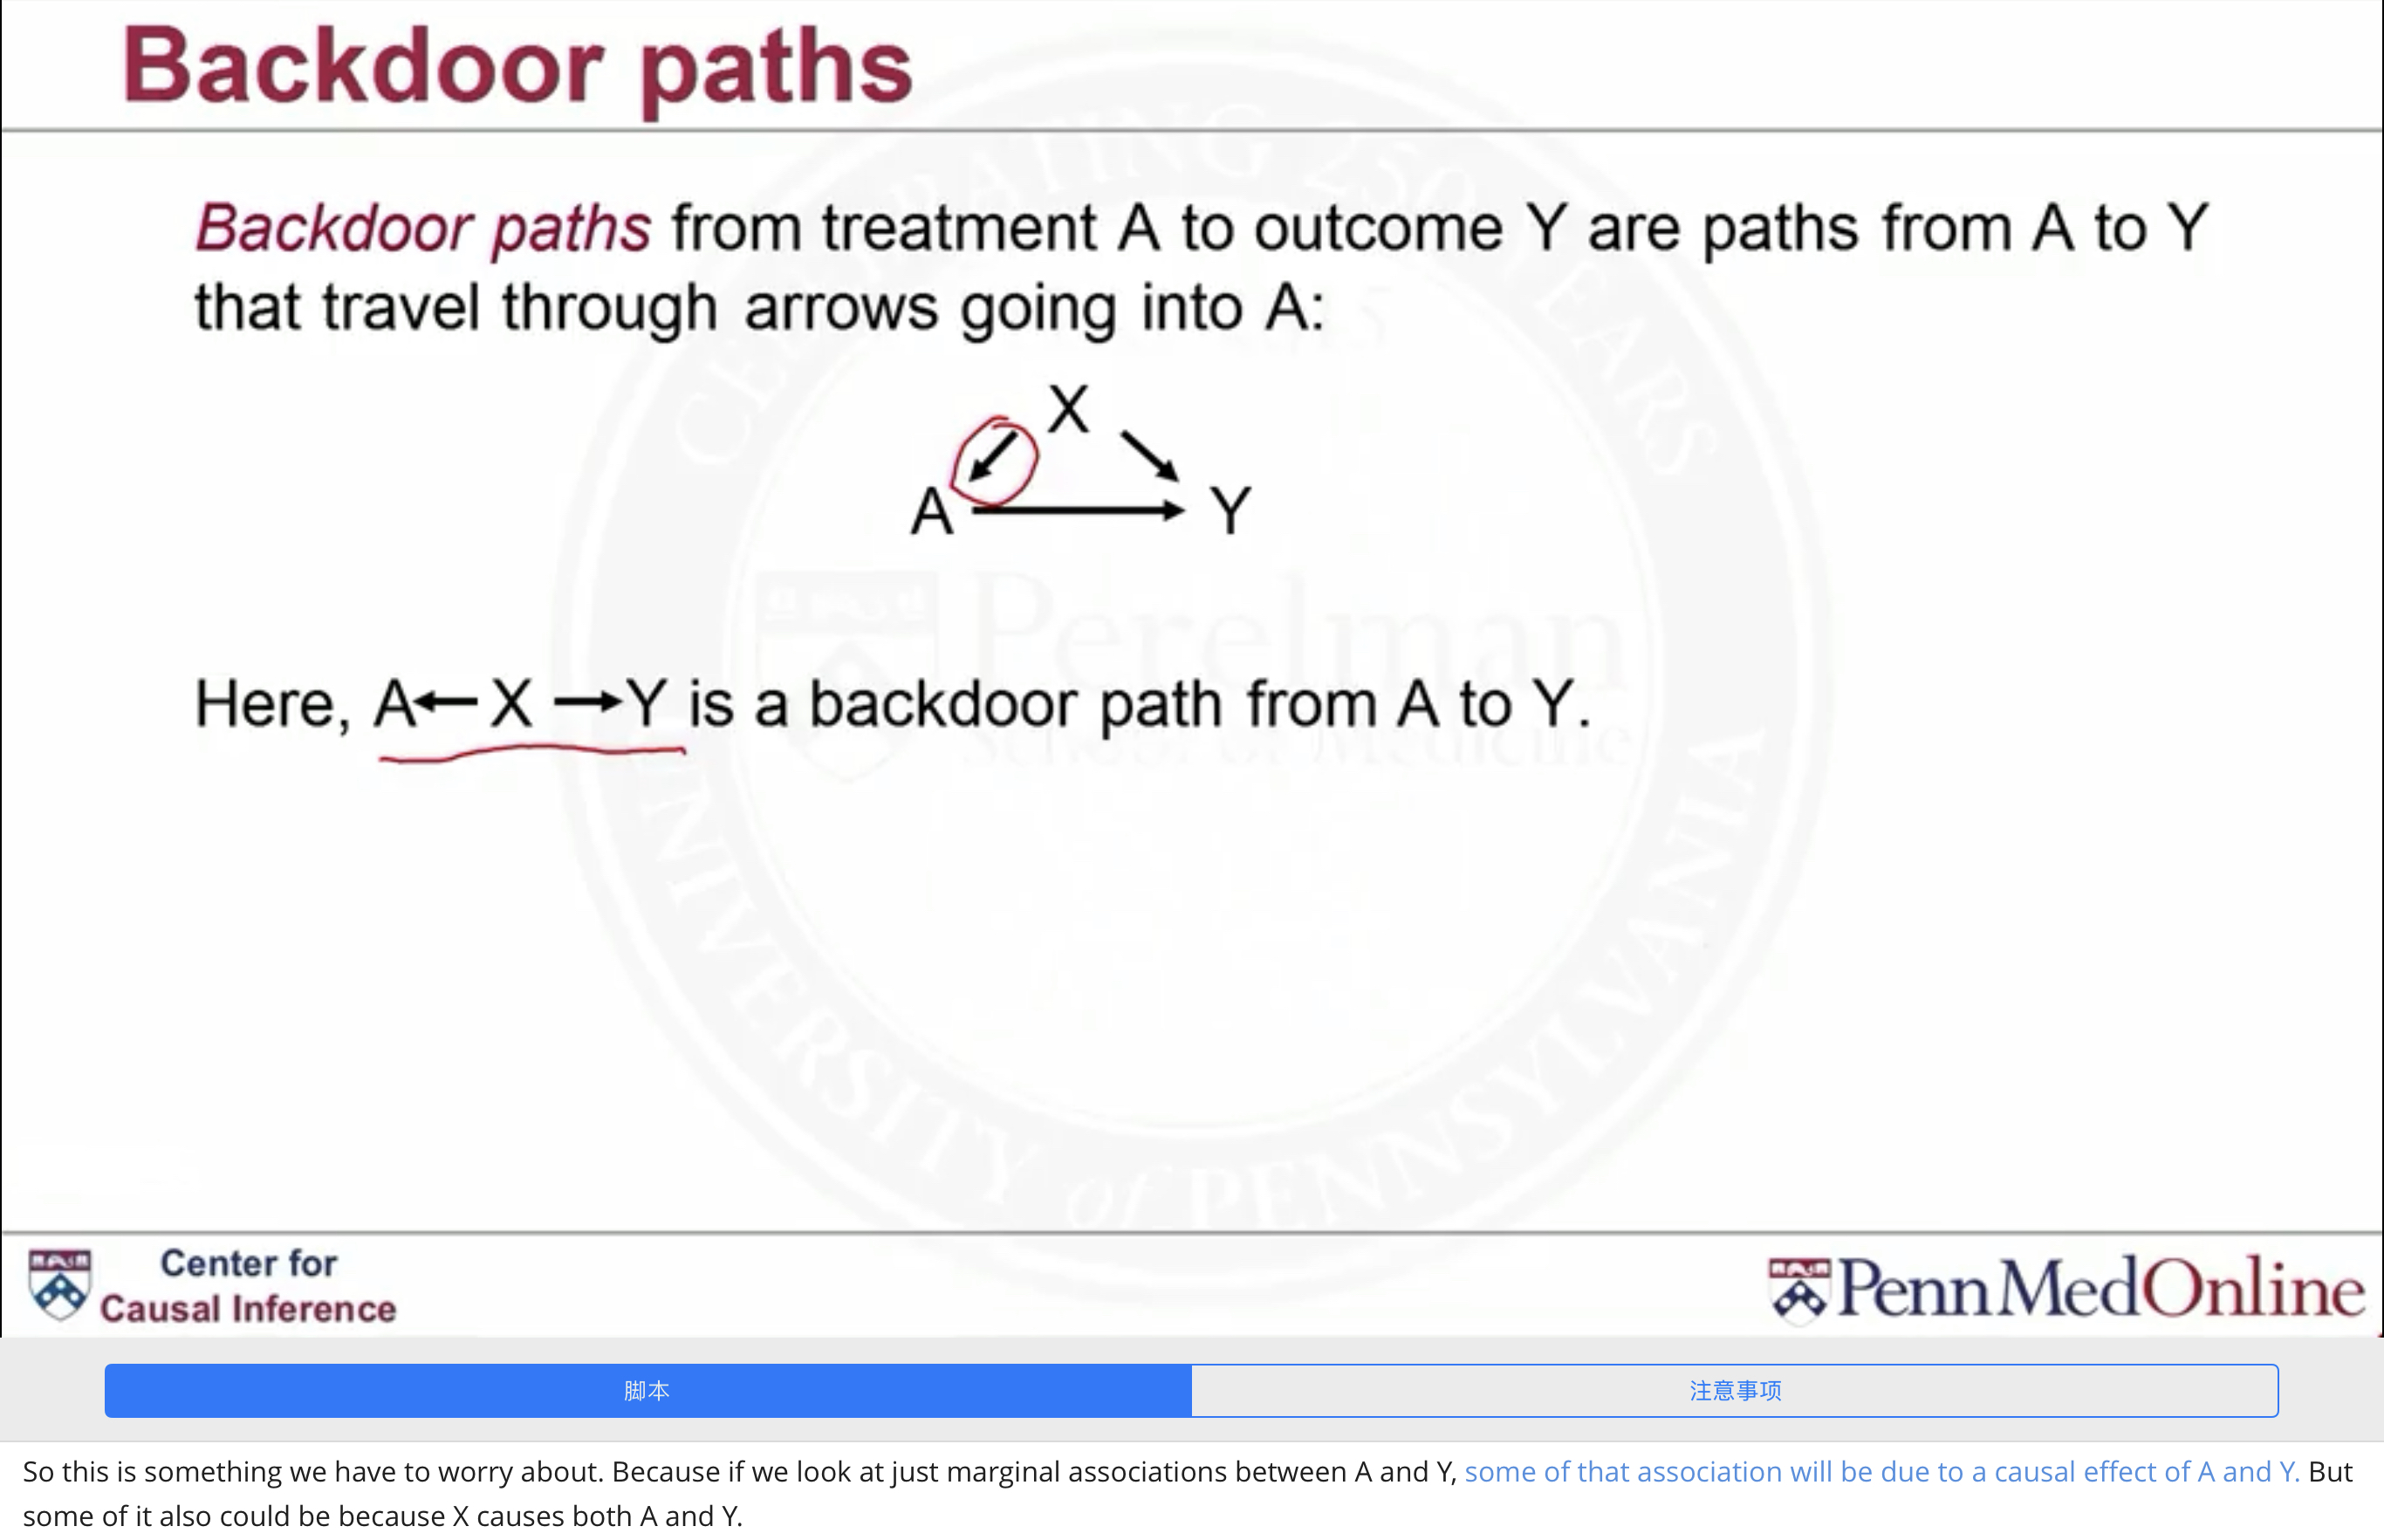
\includegraphics[width=0.8\textwidth]{figure/backdoor.jpg}
	\caption{Backdoor path}
	\label{backdoor}
\end{figure}
如果我们只关注A与Y的边缘相关的话,其中一部分相关性是由于A对Y的causal effect造成的. 但是这部分causal effect中还有一部分是由于X对A的影响造成的. 

因此backdoor path影响了A对Y的真实causal effect的估计,我们需要backdoor path加以阻隔. 

如果我们block all backdoor paths,那么就可以满足ignorability assumption: $Y^0,Y^1 \perp A|X$. 也就是说我们需要寻找一个变量集X,这个变量集里的variables可以block all backdoor paths.
	\begin{figure}[htbp]
	\setlength{\abovecaptionskip}{0pt}     %调整图片标题与图距离
	\setlength{\belowcaptionskip}{10pt}
	\vspace{-0cm}  %调整图片与上文的垂直距离
	\setlength{\abovecaptionskip}{-0cm}   %调整图片标题与图距离
	\setlength{\belowcaptionskip}{-0cm}   %调整图片标题与下文距离
	\centering
	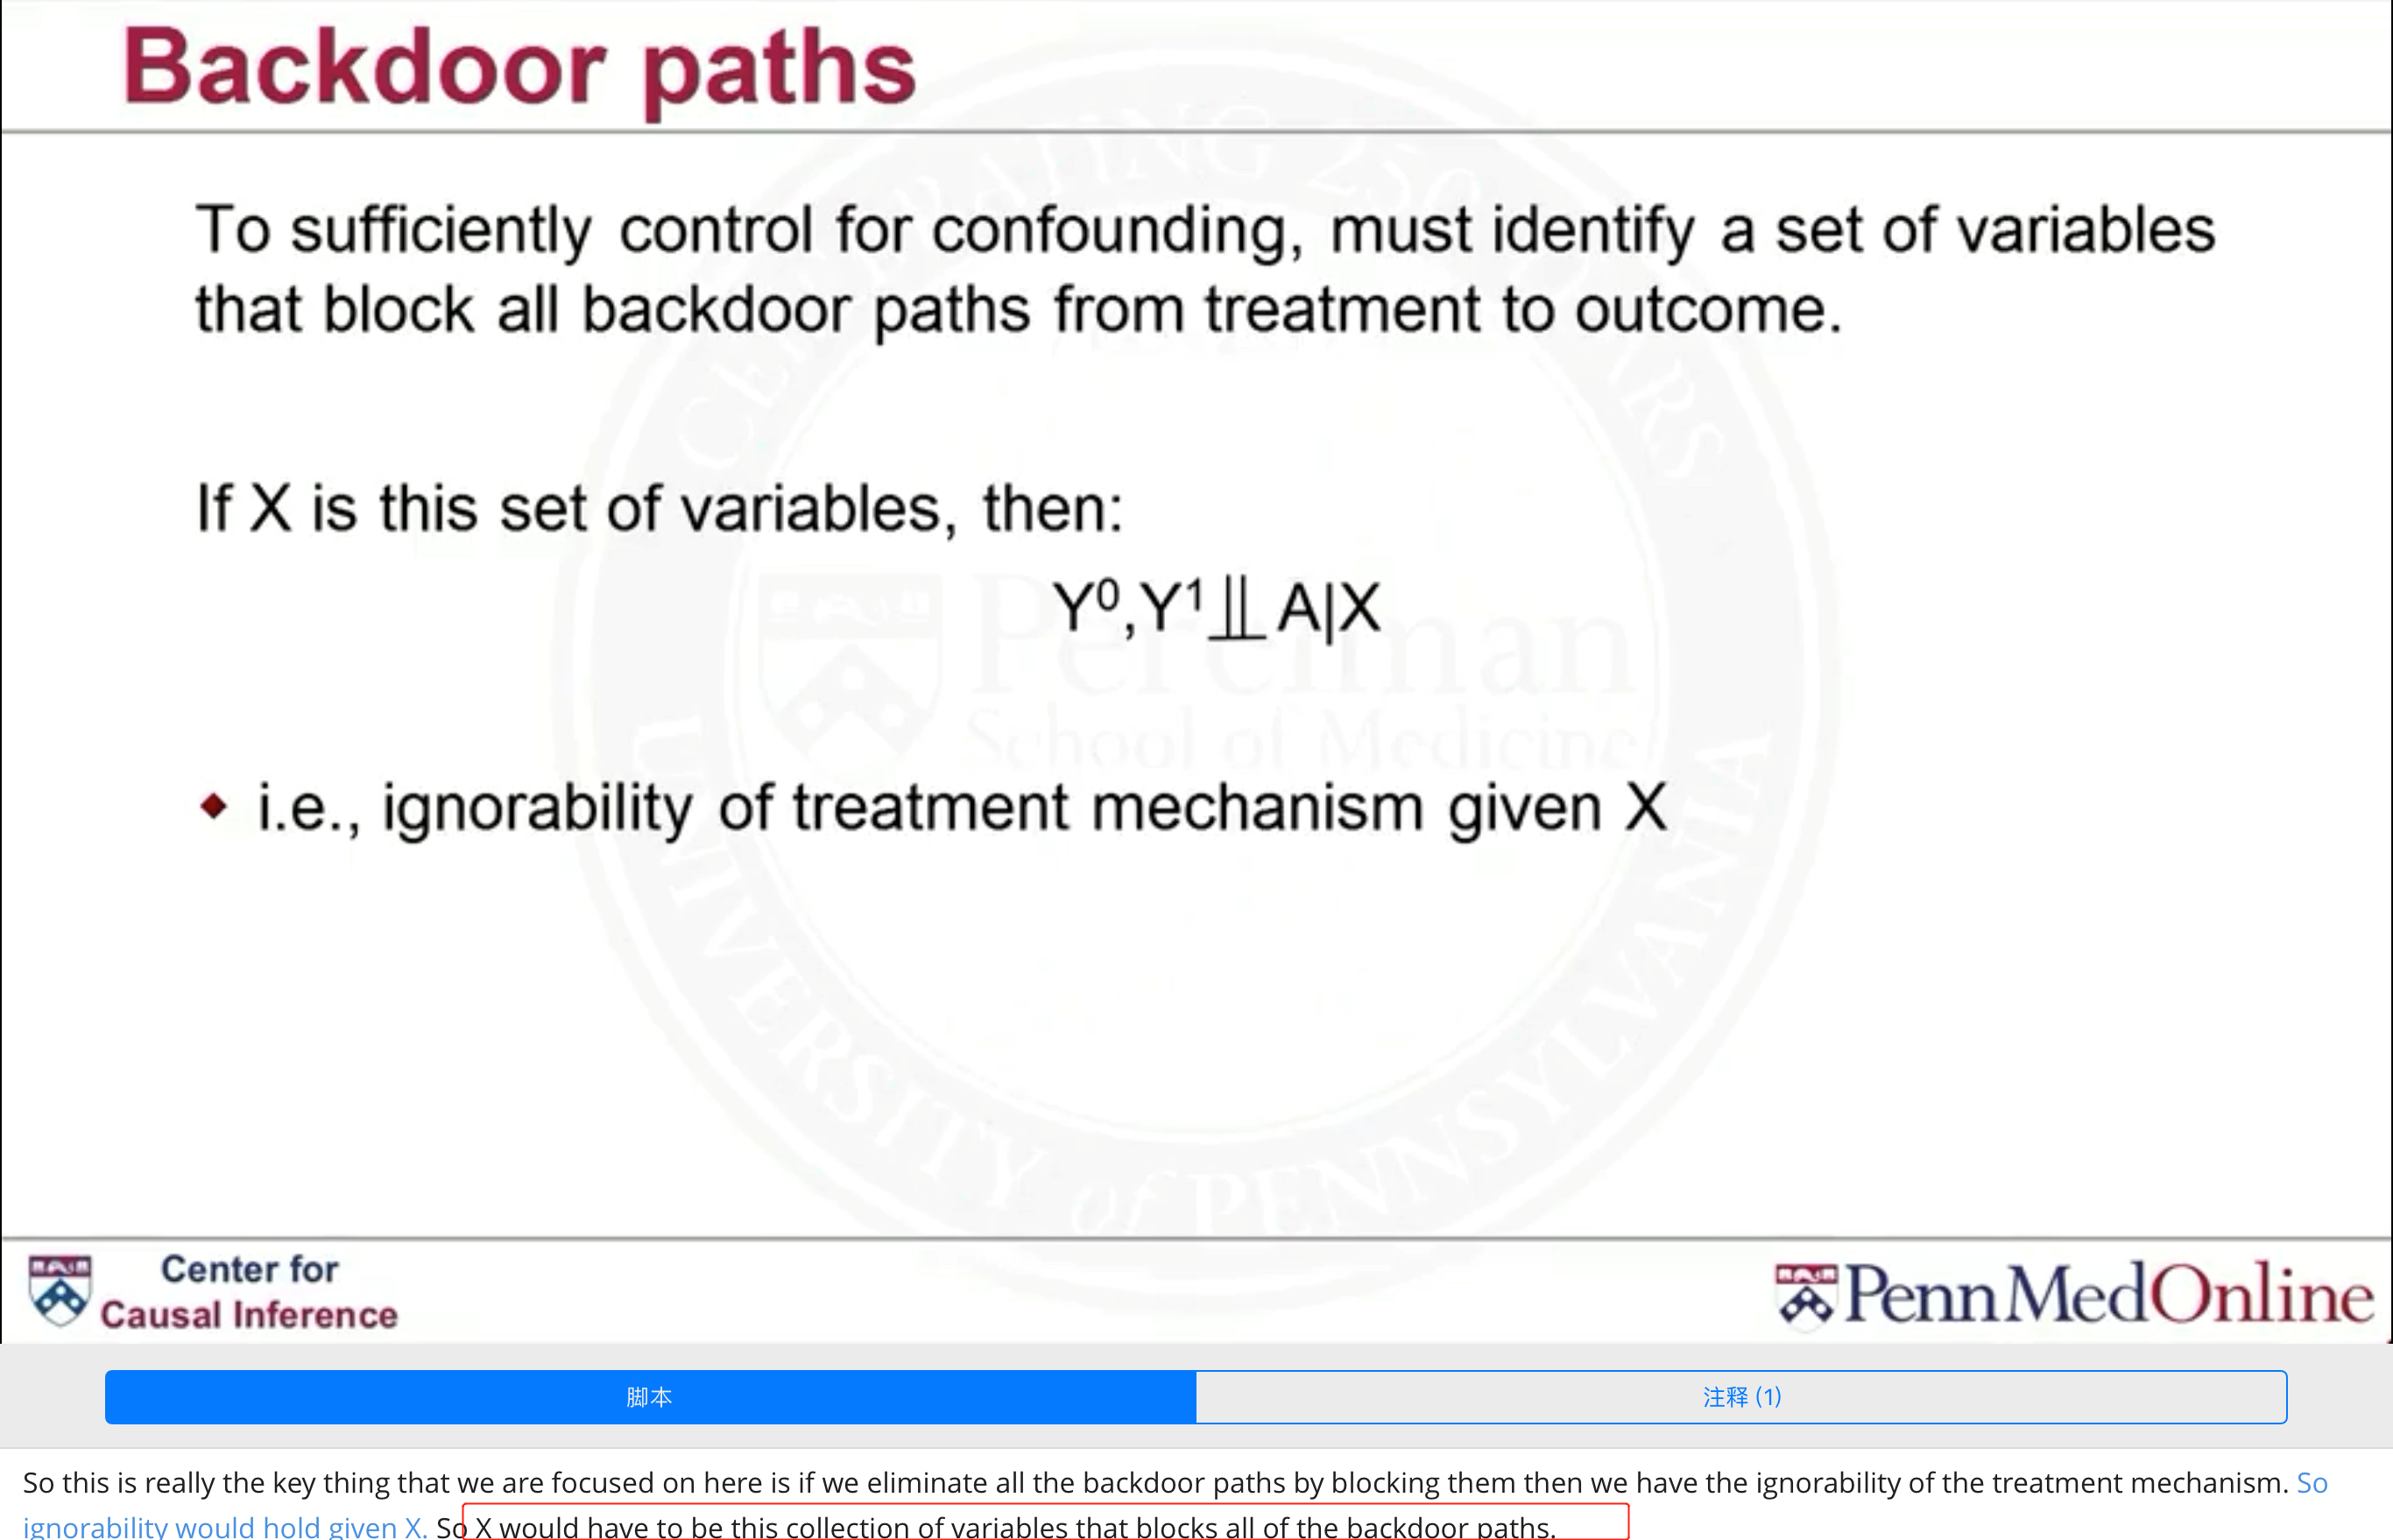
\includegraphics[width=0.8\textwidth]{figure/whyblockbackdoor.png}
	\caption{Why block Backdoor path?}
	\label{whyblockbackdoor}
    \end{figure}


\section{Backdoor path criterion}
\noindent {\bfseries Outline:}\\
1. Backdoor criterion.\\
2. When a set of variables is sufficient to control confounding?

\subsection{Backdoor path criterion}
A set of variables X is sufficient to control for confounding if:
\begin{itemize}
	\item it blocks all backdoor paths from treatment to the outcome.
	\item it does not include any descendants of treatment.
\end{itemize}
This is the {\color{red} backdoor path criterion.} 满足backdoor path criterion的变量集是{\color{red}不唯一的
}

\subsection{Examples of how to find X that are sufficient to control for confounding}
{\bfseries Example 1:}在Fig.\ref{bkdrcrtex1}中,有3个变量集满足backdoor path criterion,通常我们选择变量少的集合,比如${V}$和${W}$.
	\begin{figure}[htbp]
	\setlength{\abovecaptionskip}{0pt}     %调整图片标题与图距离
	\setlength{\belowcaptionskip}{10pt}
	\vspace{-0cm}  %调整图片与上文的垂直距离
	\setlength{\abovecaptionskip}{-0cm}   %调整图片标题与图距离
	\setlength{\belowcaptionskip}{-0cm}   %调整图片标题与下文距离
	\centering
	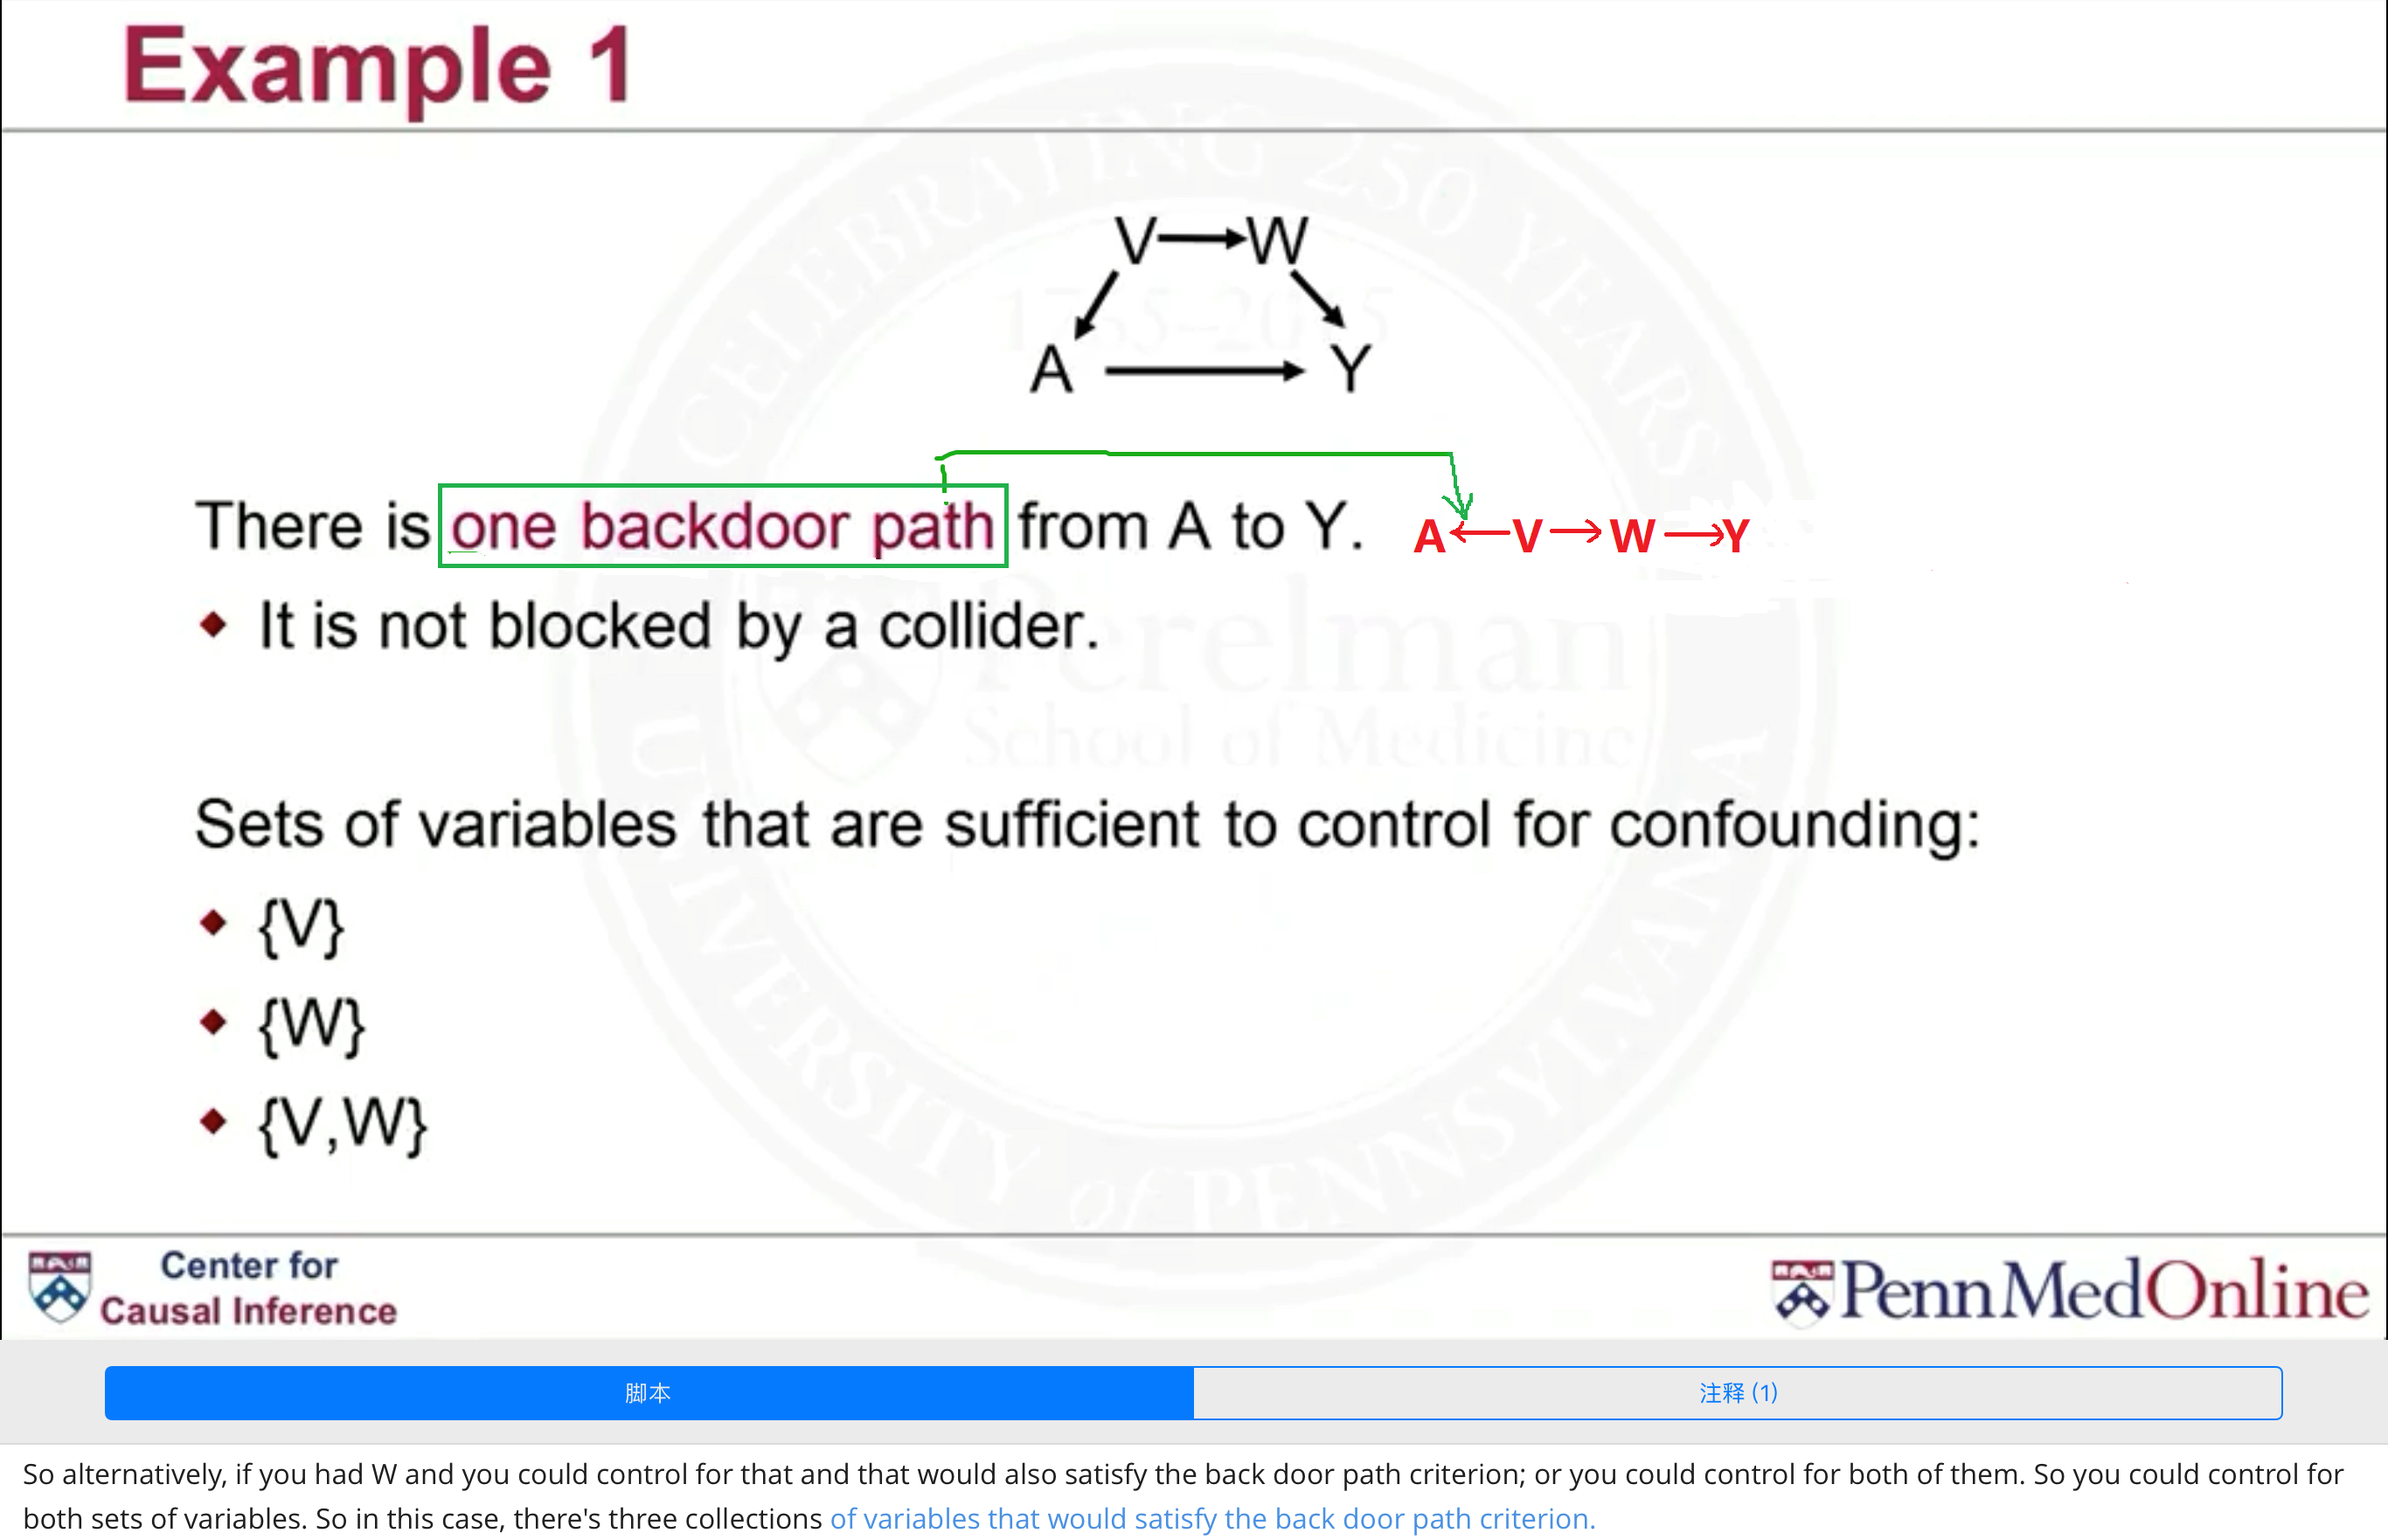
\includegraphics[width=0.8\textwidth]{figure/bkdrcrtex1.png}
	\caption{Example of backdoor path criterion(1)}
	\label{bkdrcrtex1}
\end{figure}


{\bfseries Example 2:} 
\begin{figure}[htbp]
	\setlength{\abovecaptionskip}{0pt}     %调整图片标题与图距离
	\setlength{\belowcaptionskip}{10pt}
	\vspace{-0cm}  %调整图片与上文的垂直距离
	\setlength{\abovecaptionskip}{-0cm}   %调整图片标题与图距离
	\setlength{\belowcaptionskip}{-0cm}   %调整图片标题与下文距离
	\centering
	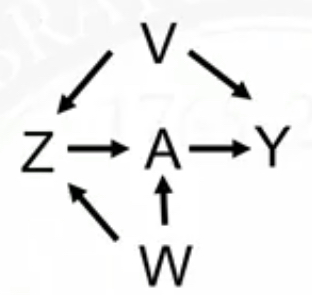
\includegraphics[width=0.2\textwidth]{figure/bckdrcrtex2.png}
	\caption{Example of backdoor path criterion((2)}
	\label{bckdrcrtex2}
\end{figure}
在Fig.\ref{bckdrcrtex2}中,我们可以找到两条backdoor paths from A to Y. 解答步骤在Fig.\ref{answerbckdrcrtex2}中详细给出.
\begin{figure}[htbp]
	\setlength{\abovecaptionskip}{0pt}     %调整图片标题与图距离
	\setlength{\belowcaptionskip}{10pt}
	\vspace{-0cm}  %调整图片与上文的垂直距离
	\setlength{\abovecaptionskip}{-0cm}   %调整图片标题与图距离
	\setlength{\belowcaptionskip}{-0cm}   %调整图片标题与下文距离
	\centering
	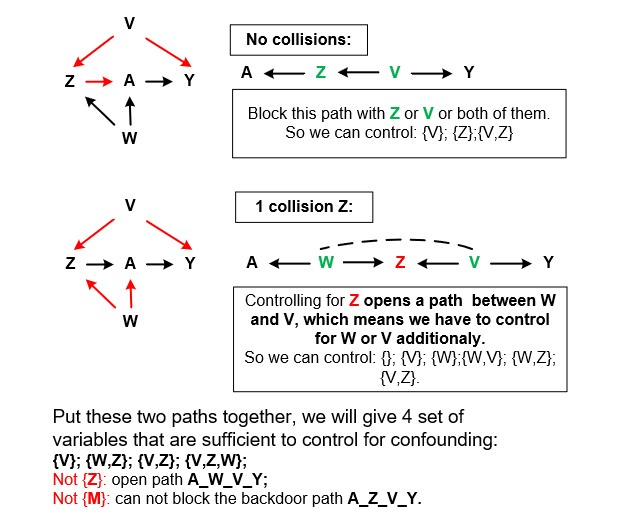
\includegraphics[width=0.8\textwidth]{figure/answerbckdrcrtex2.png}
	\caption{Solution step of example(2)}
	\label{answerbckdrcrtex2}
\end{figure}
在这个例子中,需要说明的是为什么在backdoor path:A $\longleftarrow$ W $\longrightarrow$ Z $\longleftarrow$ V $\longrightarrow$ Y上,不控制variables也可以?  这是因为这条backdoor path包含一个collider Z, 所以这条backdoor path本身就是blocked的,可以不用control任何一个变量.


{\bfseries Example 2:} 
Now we give another complicated example in Fig.\ref{bckdrcrtex3}.
\begin{figure}[h]
	\setlength{\abovecaptionskip}{0pt}     %调整图片标题与图距离
	\setlength{\belowcaptionskip}{10pt}
	\vspace{-0cm}  %调整图片与上文的垂直距离
	\setlength{\abovecaptionskip}{-0cm}   %调整图片标题与图距离
	\setlength{\belowcaptionskip}{-0cm}   %调整图片标题与下文距离
	\centering
	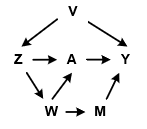
\includegraphics[width=0.2\textwidth]{figure/bckdrcrtex3.png}
	\caption{Example of backdoor path criterion((2)}
	\label{bckdrcrtex3}
\end{figure}
解答的步骤如Fig.\ref{answerbckdrcrtex3}所示. 结合所有的backdoor paths,我们可以总结出以下的sets of variables that are sufficient to control for confounding:

\begin{figure}[htbp]
	\setlength{\abovecaptionskip}{0pt}     %调整图片标题与图距离
	\setlength{\belowcaptionskip}{10pt}
	\vspace{-0cm}  %调整图片与上文的垂直距离
	\setlength{\abovecaptionskip}{-0cm}   %调整图片标题与图距离
	\setlength{\belowcaptionskip}{-0cm}   %调整图片标题与下文距离
	\centering
	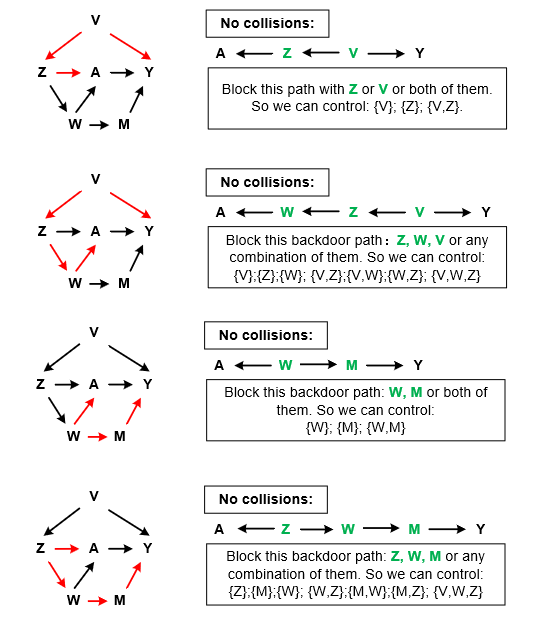
\includegraphics[width=0.8\textwidth]{figure/answerbckdrcrtex3.png}
	\caption{Solution step of example(3)}
	\label{answerbckdrcrtex3}
\end{figure}
Put these two paths together, we will give   sets of variables that are sufficient to control for confounding:$\{V,M\},\{V,W\},\{Z,W\},\{Z,M\}; \{V,W,M\},\{V,Z,M\},\{V,Z,W\}; \{V,Z,W,M\}$.


\subsection{Conclusion}
上面所给出的例子都是基于正确的DAG,有了正确的DAG,我们才知道应该控制哪些变量. 问题在于:在实际问题中我们一开始并不知道真实的DAG是什么样子的. 此时如何构造DAG?进一步,如果构造的DAG不一定正确该怎么办?

我们关注的问题是:在DAG有小幅变动的情况下,confoundr control仍然有效. 或者说:If the DAG looks slightly different, can we still sufficiently control for confounding? 
\begin{figure}[htbp]
	\setlength{\abovecaptionskip}{0pt}     %调整图片标题与图距离
	\setlength{\belowcaptionskip}{10pt}
	\vspace{-0cm}  %调整图片与上文的垂直距离
	\setlength{\abovecaptionskip}{-0cm}   %调整图片标题与图距离
	\setlength{\belowcaptionskip}{-0cm}   %调整图片标题与下文距离
	\centering
	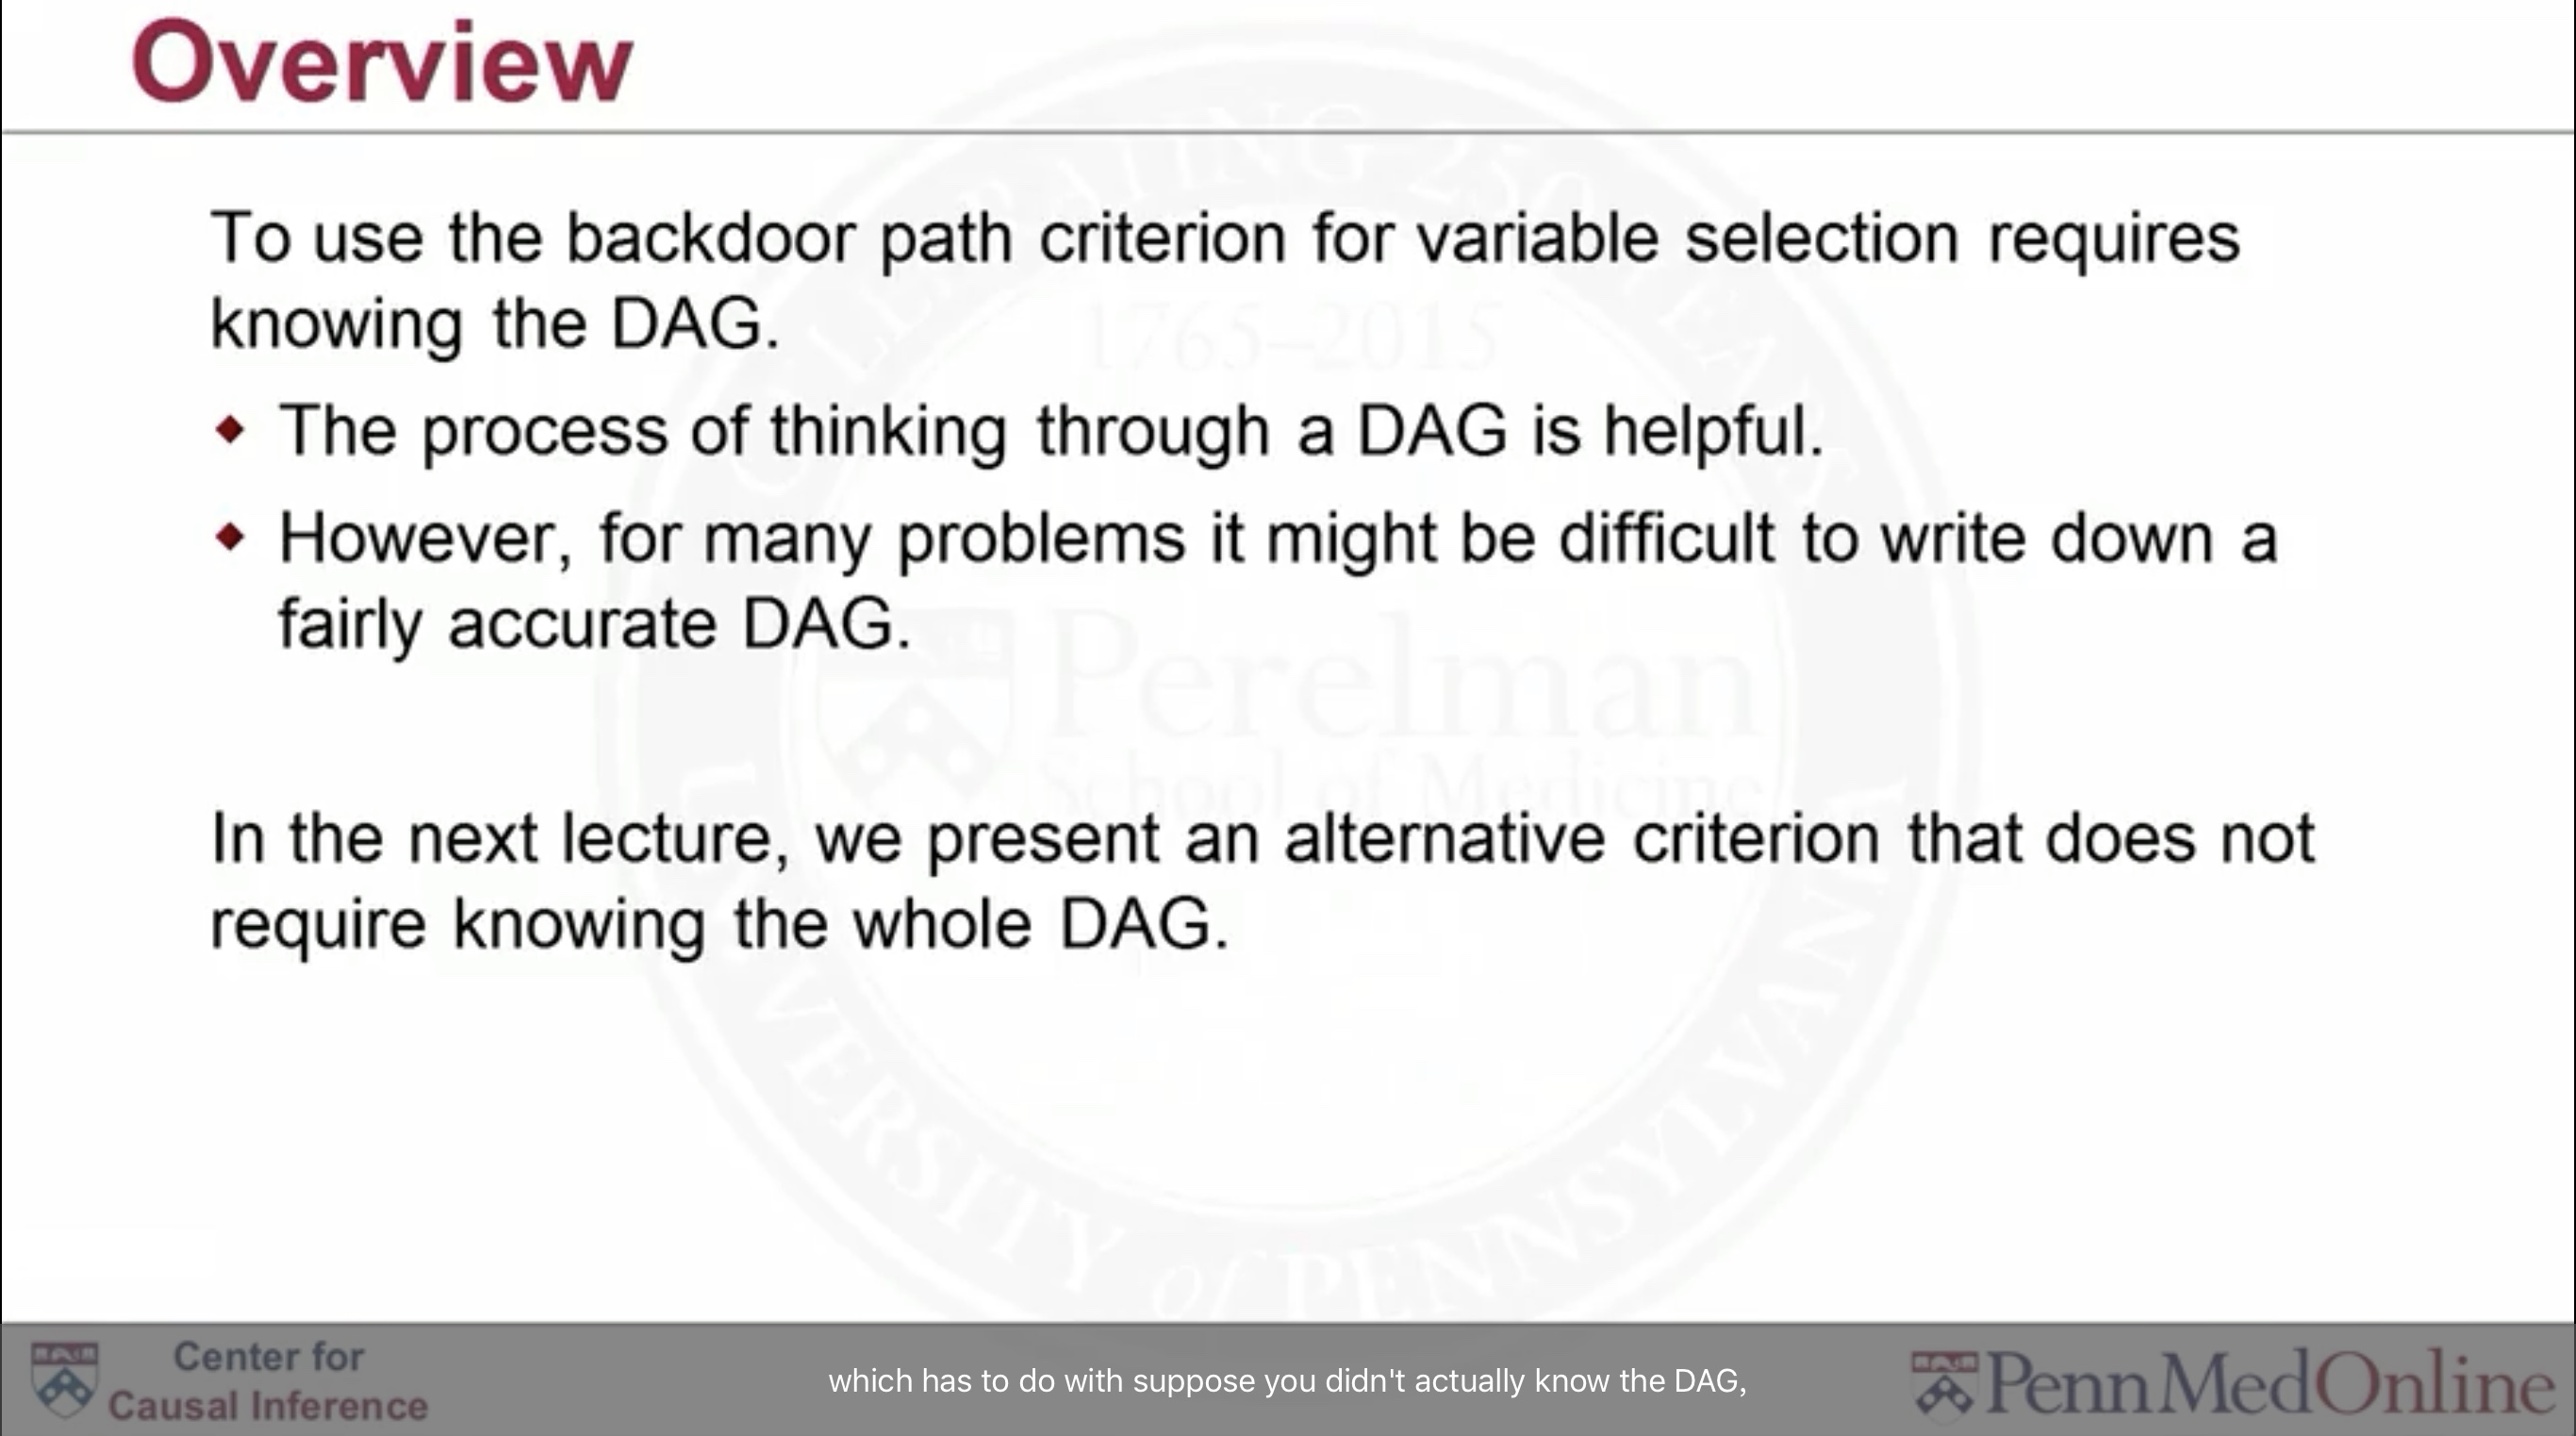
\includegraphics[width=0.8\textwidth]{figure/conclusionbdc.jpg}
	\caption{Conclusion of backdoor path criterion}
	\label{conclusionbdc}
\end{figure}

\section{Disjunctive cause criterion}
\noindent {\bfseries Outline:}\\
1. Disjunctive cause criterion. \\
2. The relationship between \r{disjunctive cause criterion} and \r{backdoor path criterion.} \\
3. {\bfseries Comparasion} of \r{pre-treatment covariates} and \r{disjunctive cause criterion.}

\subsection{Disjunctive cause criterion}
{\bfseries Disjunctive cause criterion: } Control for all(observed) causes of the exposure, the outcome, or both. This criterion was put forward to choose variables to control for(VanderWeele 2011).

\paragraph{The advantage of disjunctive cause criterion.} One \r{has no need to know the whole graph}, usually we can not know the whole graph. Instead, we \r{only need to identify the variables that affect exposure or outcome.}

\subsection{Property}
The property of disjunctive cause criterion shows its  relationship with \r{backdoor path criterion.}
\begin{thm}
	If there is a set of variables that satisfy the backdoor path criterion, then the variables selected based on the disjunctive cause criterion will be sufficient to control for confounding.
\end{thm}

这个定理告诉我们,如果存在满足backdoor path criterion的观测变量集,那么基于disjunctive cause criterion选择的变量将足够控制confounding.

\subsection{Pre-treatment covariates}
Here we don't know what the DAG is, but we might have some information about observed variables.  

One strategy is using all observed pre-treatment covariates. 

\begin{ex}
	\label{exdcc1}
	Observed pre-treatment variables:${M,W,V}$;
	Unobserved pre-treatment variables: ${U_1,U_2}$;
	Suppose we know that W and V are the causes of A, Y or both. M is not a cuase of either A or Y. Fig.\ref{exdcc} is the causal graph of this example.
 Then compare 2 methods for selecting variables to control: 
 \begin{itemize}
 	\item Use all observed pre-treatment covariate: ${M,W,V}$. The set of variables satisfies the backdoor path criterion.
 	\item Use variables based on dcc: ${W,V}$. The set of variables satisfies the backdoor path criterion.
 \end{itemize}

在这种情况下,两种方法得到的set of variables are sufficient to control for confounding.
\end{ex}

\begin{figure}[htbp]
	\setlength{\abovecaptionskip}{0pt}     %调整图片标题与图距离
	\setlength{\belowcaptionskip}{10pt}
	\vspace{-0cm}  %调整图片与上文的垂直距离
	\setlength{\abovecaptionskip}{-0cm}   %调整图片标题与图距离
	\setlength{\belowcaptionskip}{-0cm}   %调整图片标题与下文距离
	\centering
	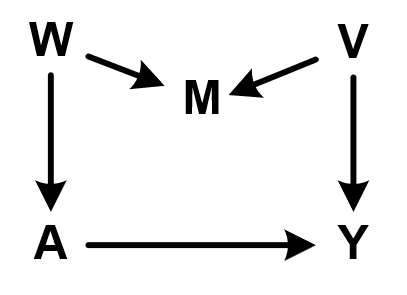
\includegraphics[width=0.2\textwidth]{figure/exdcc.png}
	\caption{Hypothetical Dag 2}
	\label{exdcc}
\end{figure}

需要强调的是,像{\bfseries Example\ref{exdcc1}}这样,两种准则都适用的情况并不常见,下面我们将给出两个例子,说明当观测变量刚好是未观测变量的collider时,控制pre-treatment变量和Disjunctive cause criterion将会失效. 
\begin{figure}[htbp]
	\setlength{\abovecaptionskip}{0pt}     %调整图片标题与图距离
	\setlength{\belowcaptionskip}{10pt}
	\vspace{-0cm}  %调整图片与上文的垂直距离
	\setlength{\abovecaptionskip}{-0cm}   %调整图片标题与图距离
	\setlength{\belowcaptionskip}{-0cm}   %调整图片标题与下文距离
	\centering
	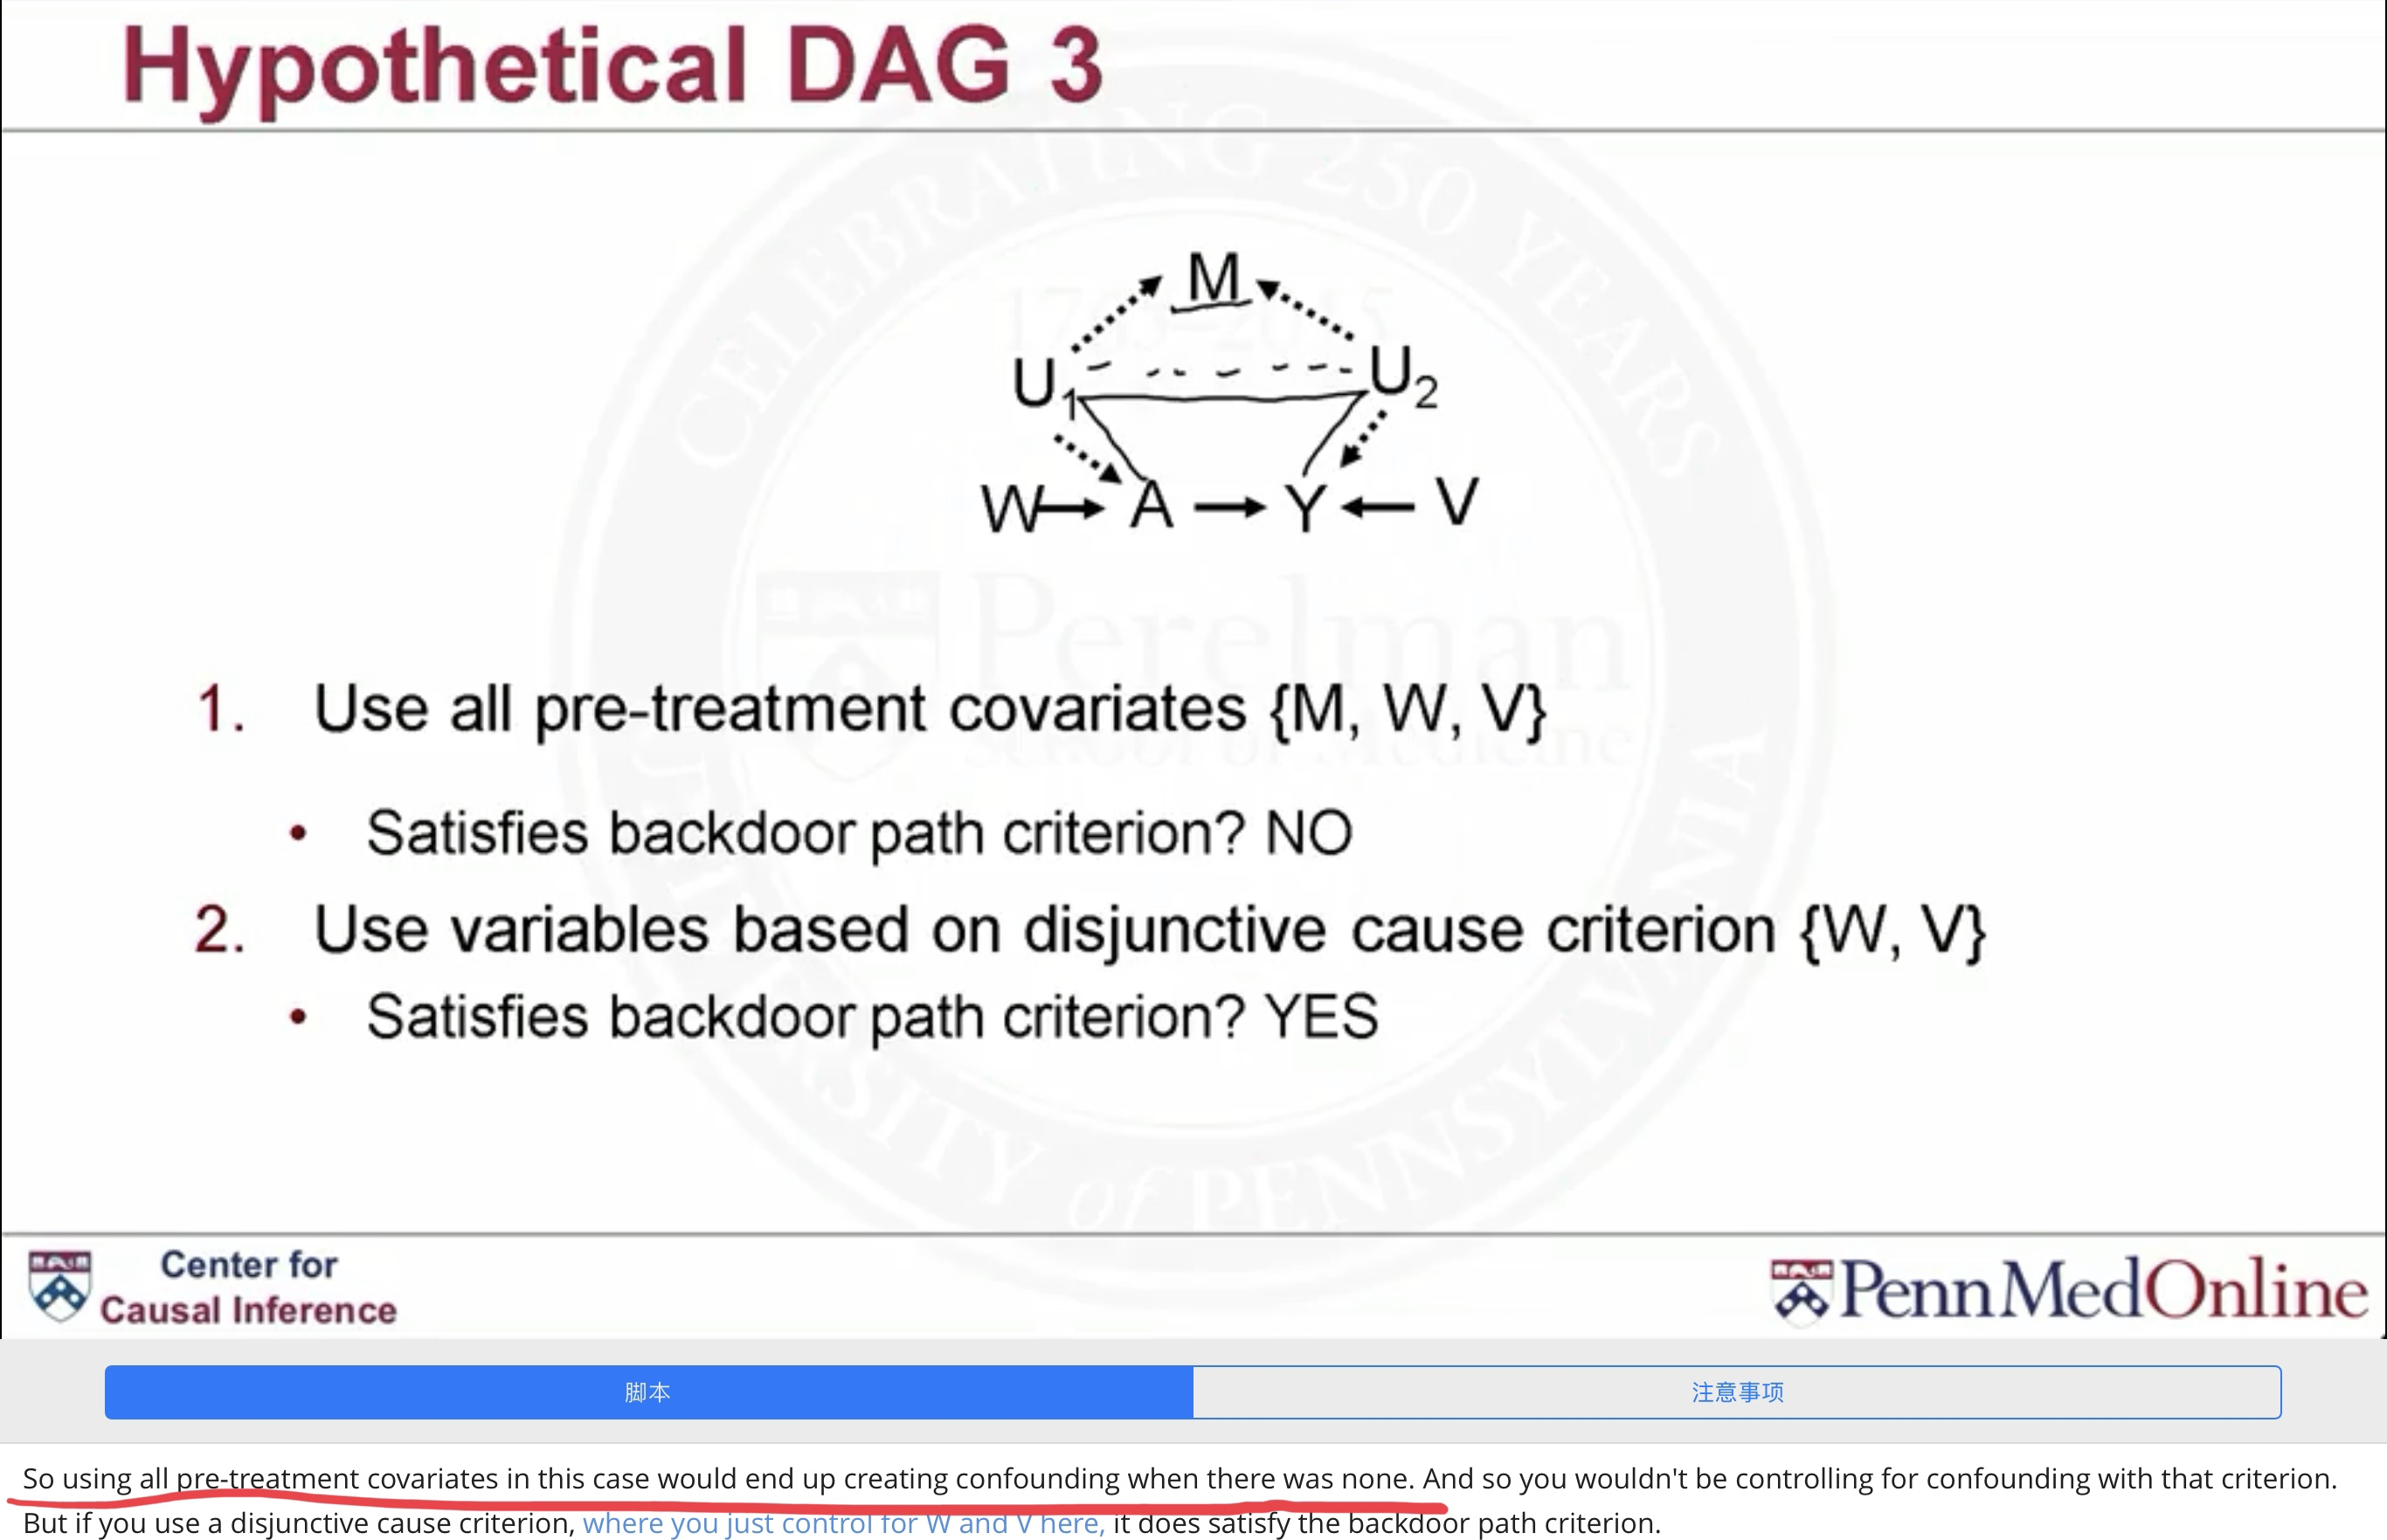
\includegraphics[width=0.6\textwidth]{figure/dccdag3.jpg}
	\caption{Hypothetical Dag 3}
	\label{dccdag3}
\end{figure}
	
\begin{figure}[htbp]
	\setlength{\abovecaptionskip}{0pt}     %调整图片标题与图距离
	\setlength{\belowcaptionskip}{10pt}
	\vspace{-0cm}  %调整图片与上文的垂直距离
	\setlength{\abovecaptionskip}{-0cm}   %调整图片标题与图距离
	\setlength{\belowcaptionskip}{-0cm}   %调整图片标题与下文距离
	\centering
	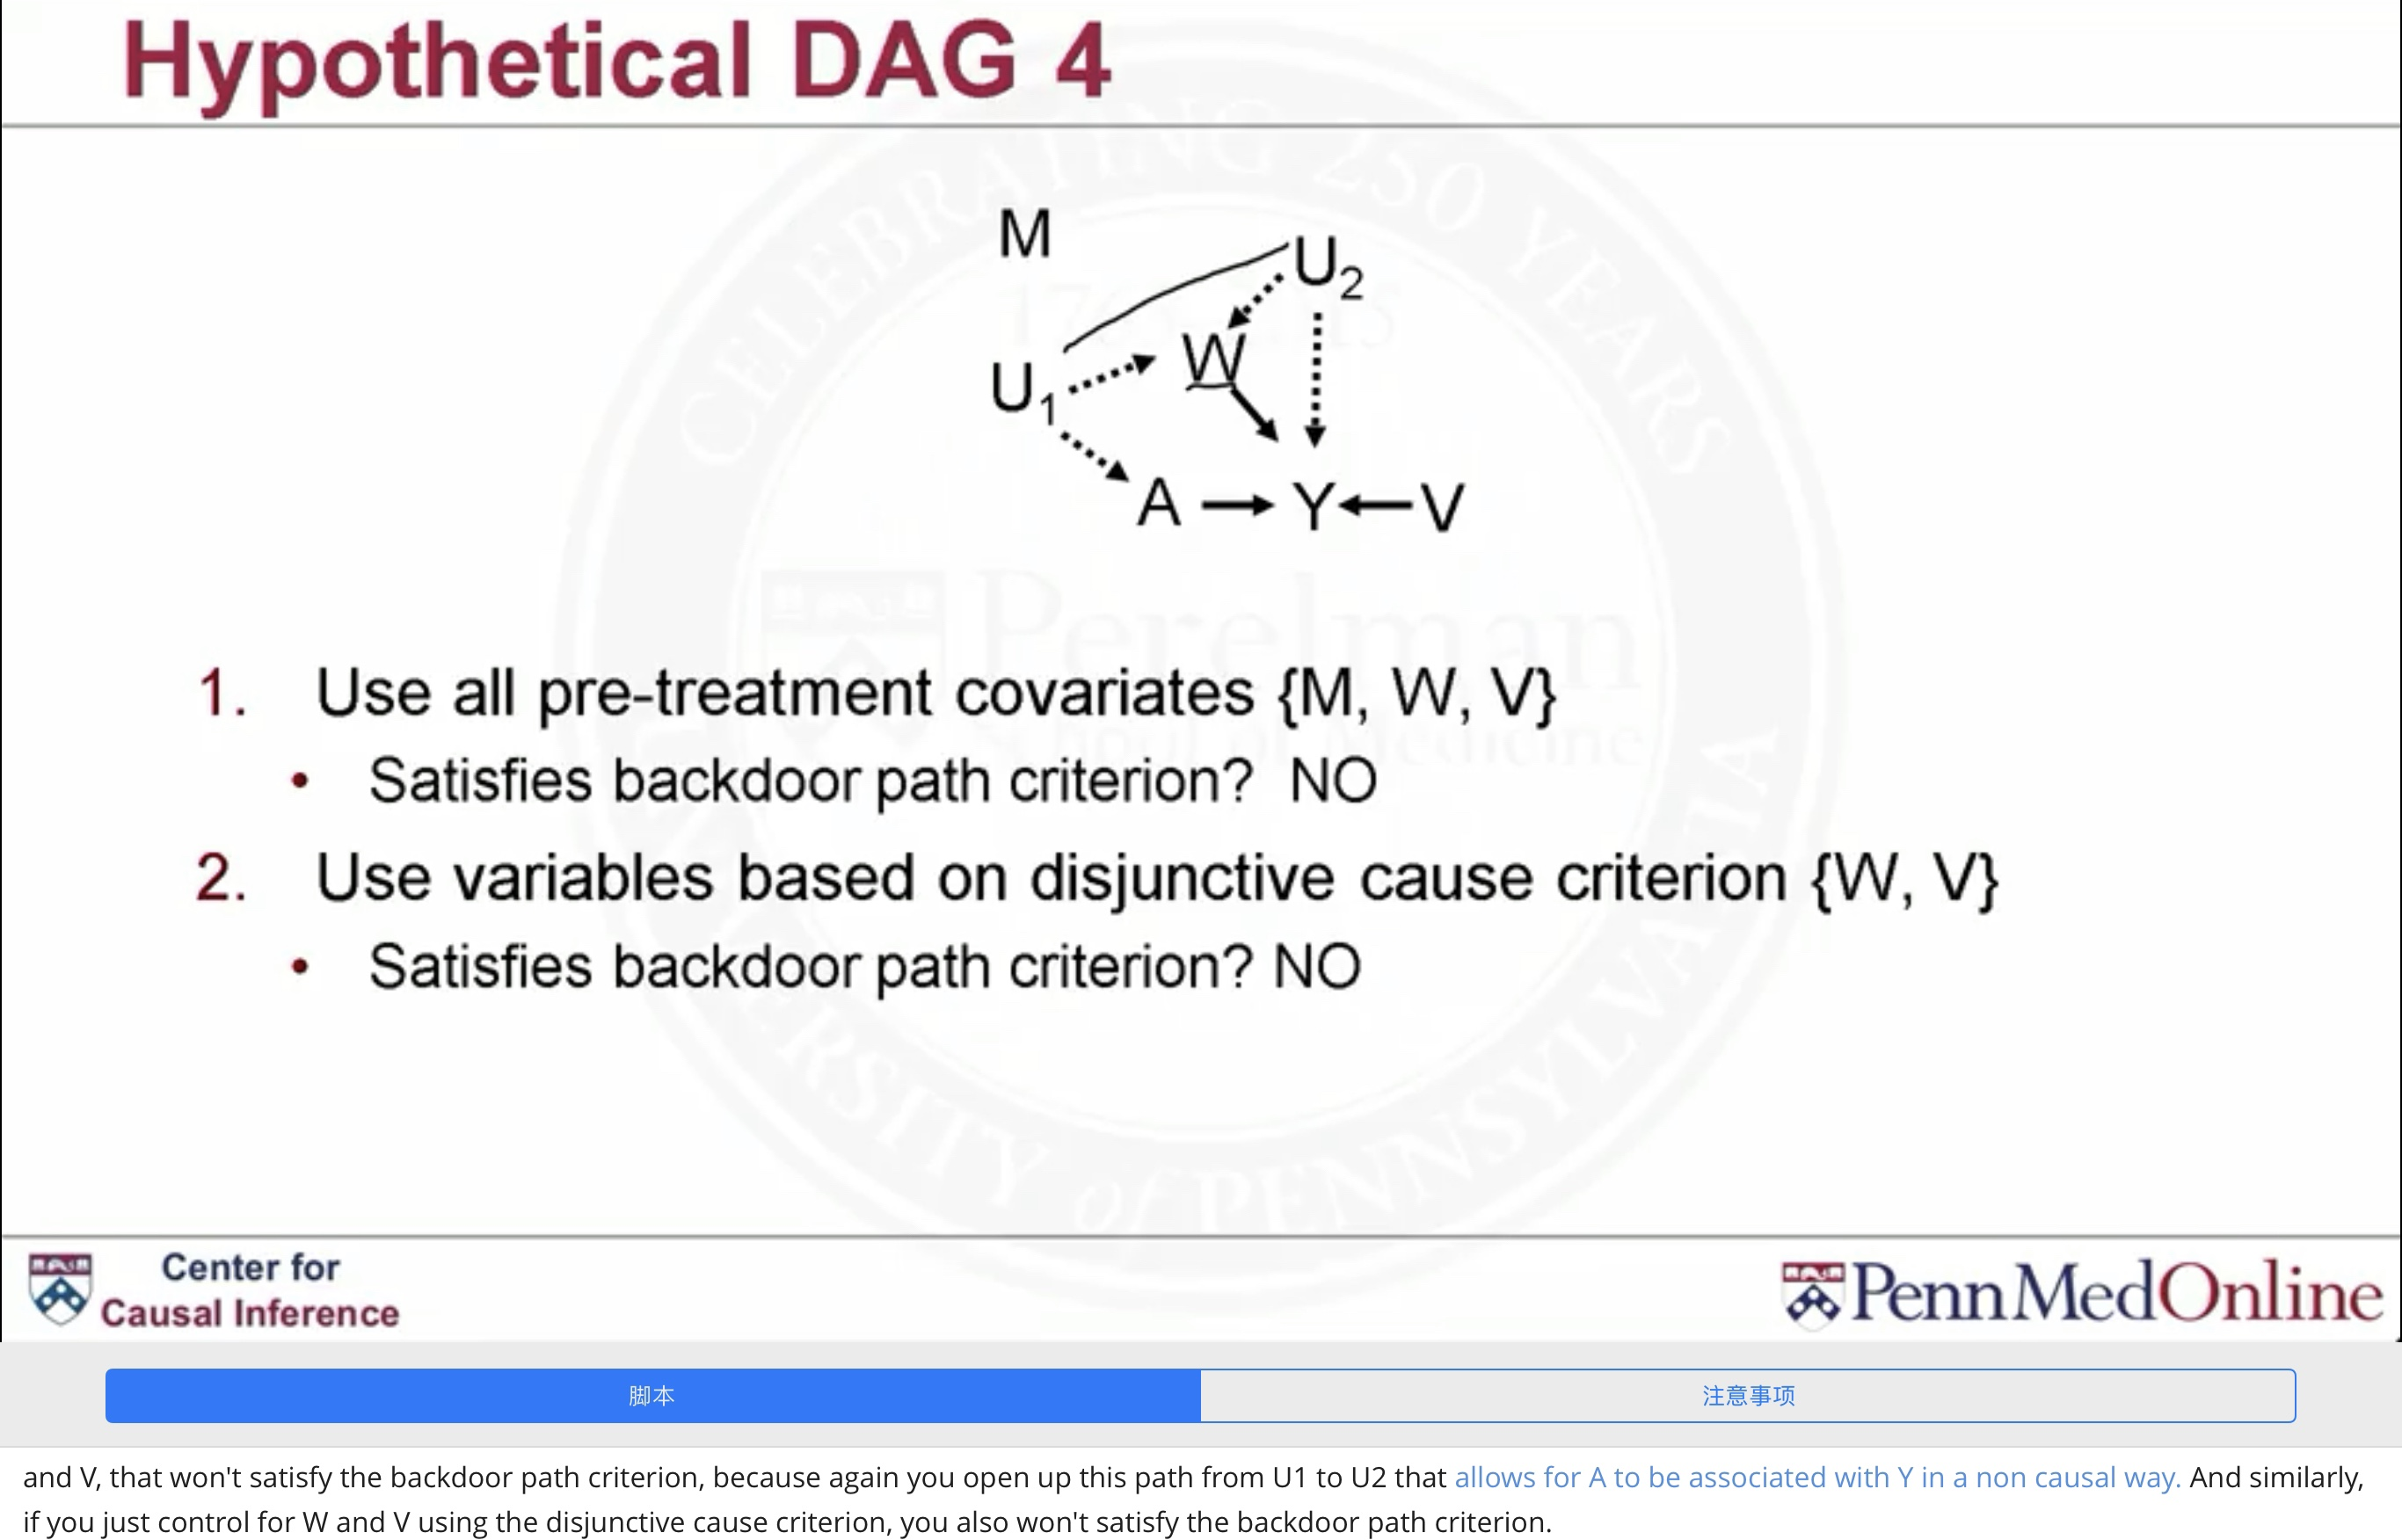
\includegraphics[width=0.6\textwidth]{figure/dccdag4.jpg}
	\caption{Hypothetical Dag 4}
	\label{dccdag4}
\end{figure}	
















